\chapter{Additional plots and tables} \label{appB:additional}

%%%%%%%%%%%%%%%%%%%%%%%%%%%%%%%%%%%%%%%%%%%%%%%%%%%%%%%%%%%%%%%%%%%%%%%
%%%%%%%%%%%%%%%%%%%%%%%%%%%%%%%%%%%%%%%%%%%%%%%%%%%%%%%%%%%%%%%%%%%%%%%

\section{Chapter 3: Bayesian estimation} \label{appB1:chapter3}

\subsection{To center or not to center} \label{appB1:noncenter}
%
\begin{figure}[H]
	\centering
	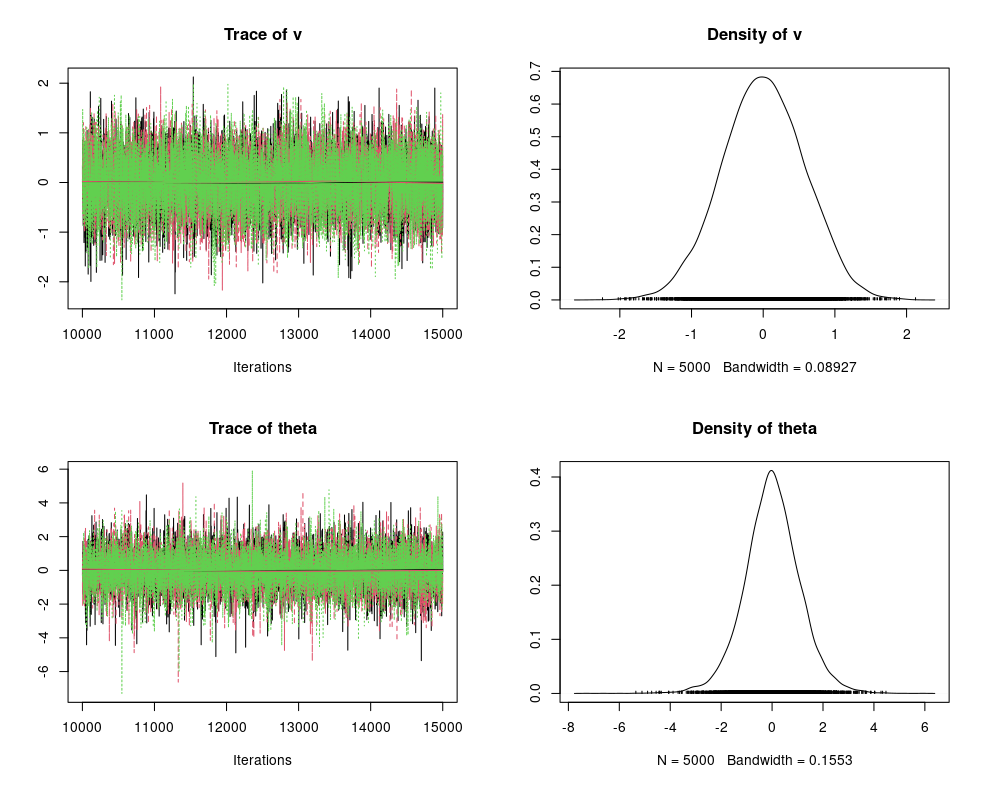
\includegraphics[width=1\linewidth]{1_jags_CE_simple}
	%
	\caption[The Devil's funnel. Centered Parametrization. JAGS]%
	{The Devil's funnel. Centered Parametrization implemented in JAGS. It shows the traceplot and distribution of the parameters of interest.}
	\label{fig:devil_CE_simple_jags}
\end{figure}
%
\begin{figure}[H]
	\centering
	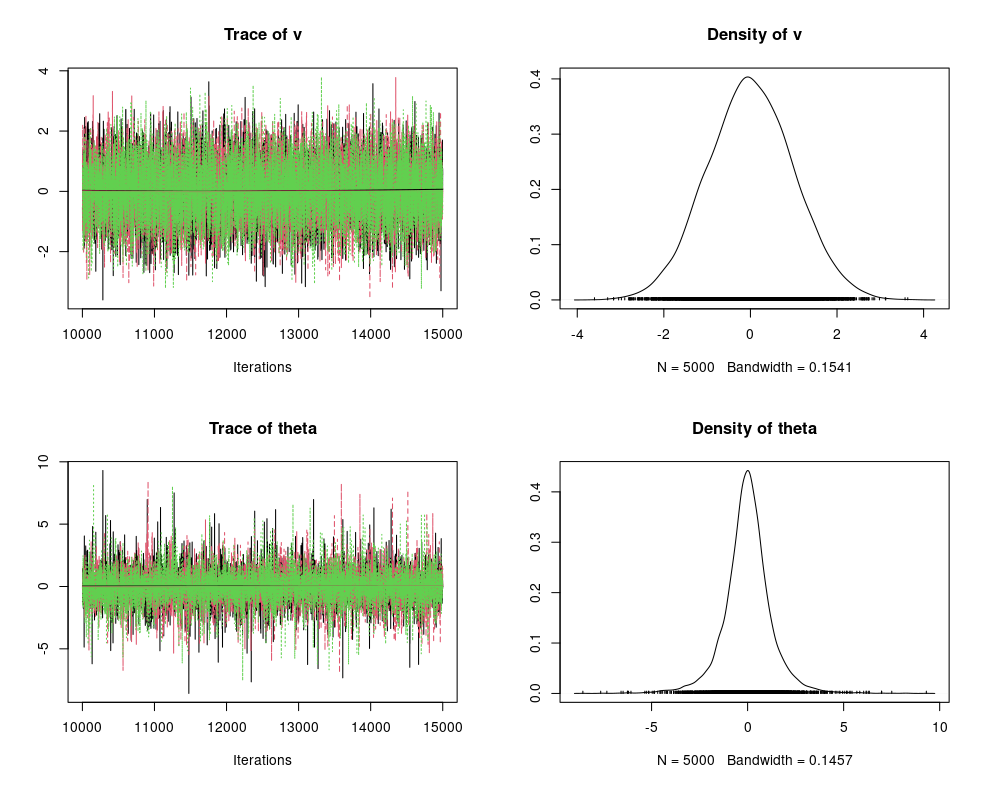
\includegraphics[width=1\linewidth]{2_jags_CE_priors}
	%
	\caption[The Devil's funnel. Centered Parametrization with mildly informative priors. JAGS]%
	{The Devil's funnel. Centered Parametrization with mildly informative priors implemented in JAGS. It shows the traceplot and distribution of the parameters of interest.}
	\label{fig:devil_CE_prior_jags}
\end{figure}
%
\begin{figure}[H]
	\centering
	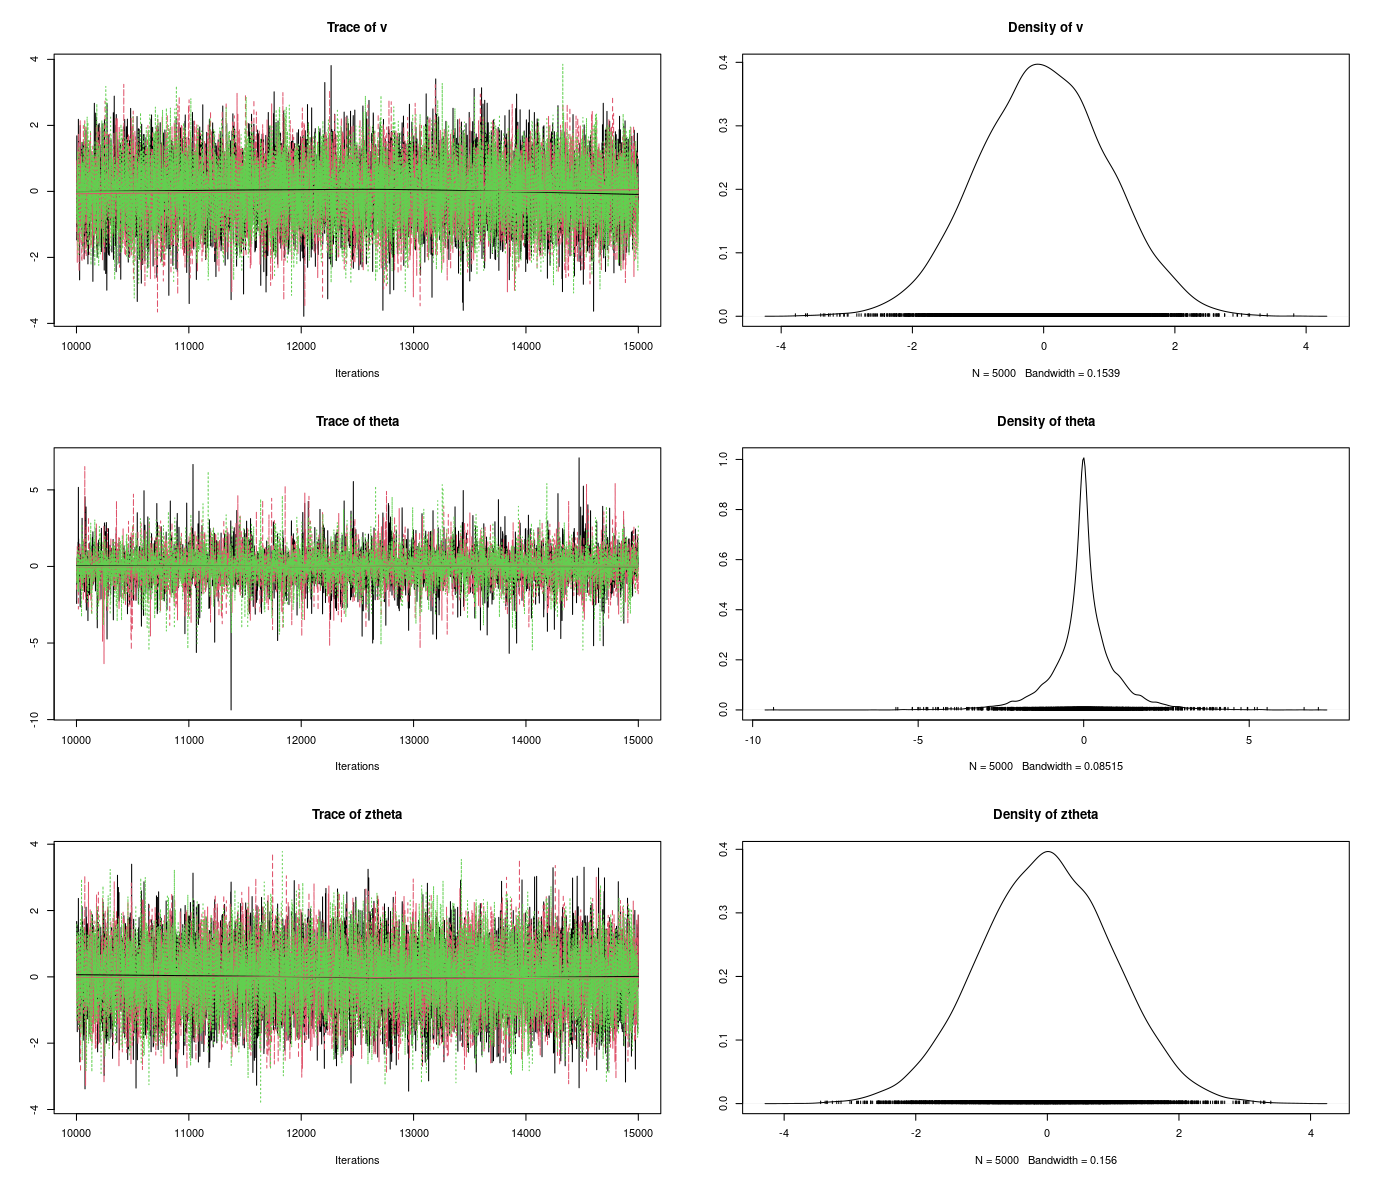
\includegraphics[width=1\linewidth]{3_jags_NC}
	%
	\caption[The Devil's funnel. Non-Centered Parametrization. JAGS]%
	{The Devil's funnel. Non-Centered Parametrization implemented in JAGS. It shows the traceplot and distribution of the parameters of interest.}
	\label{fig:devil_CE_NC_jags}
\end{figure}

%%%%%%%%%%%%%%%%%%%%%%%%%%%%%%%%%%%%%%%%%%%%%%%%%%%%%%%%%%%%%%%%%%%%%%%


%%%%%%%%%%%%%%%%%%%%%%%%%%%%%%%%%%%%%%%%%%%%%%%%%%%%%%%%%%%%%%%%%%%%%%%
%%%%%%%%%%%%%%%%%%%%%%%%%%%%%%%%%%%%%%%%%%%%%%%%%%%%%%%%%%%%%%%%%%%%%%%


\section{Chapter 4: Simulation study} \label{appB2:chapter4}

\subsection{Prior elicitation}
%
\begin{figure}[H]
	\centering
	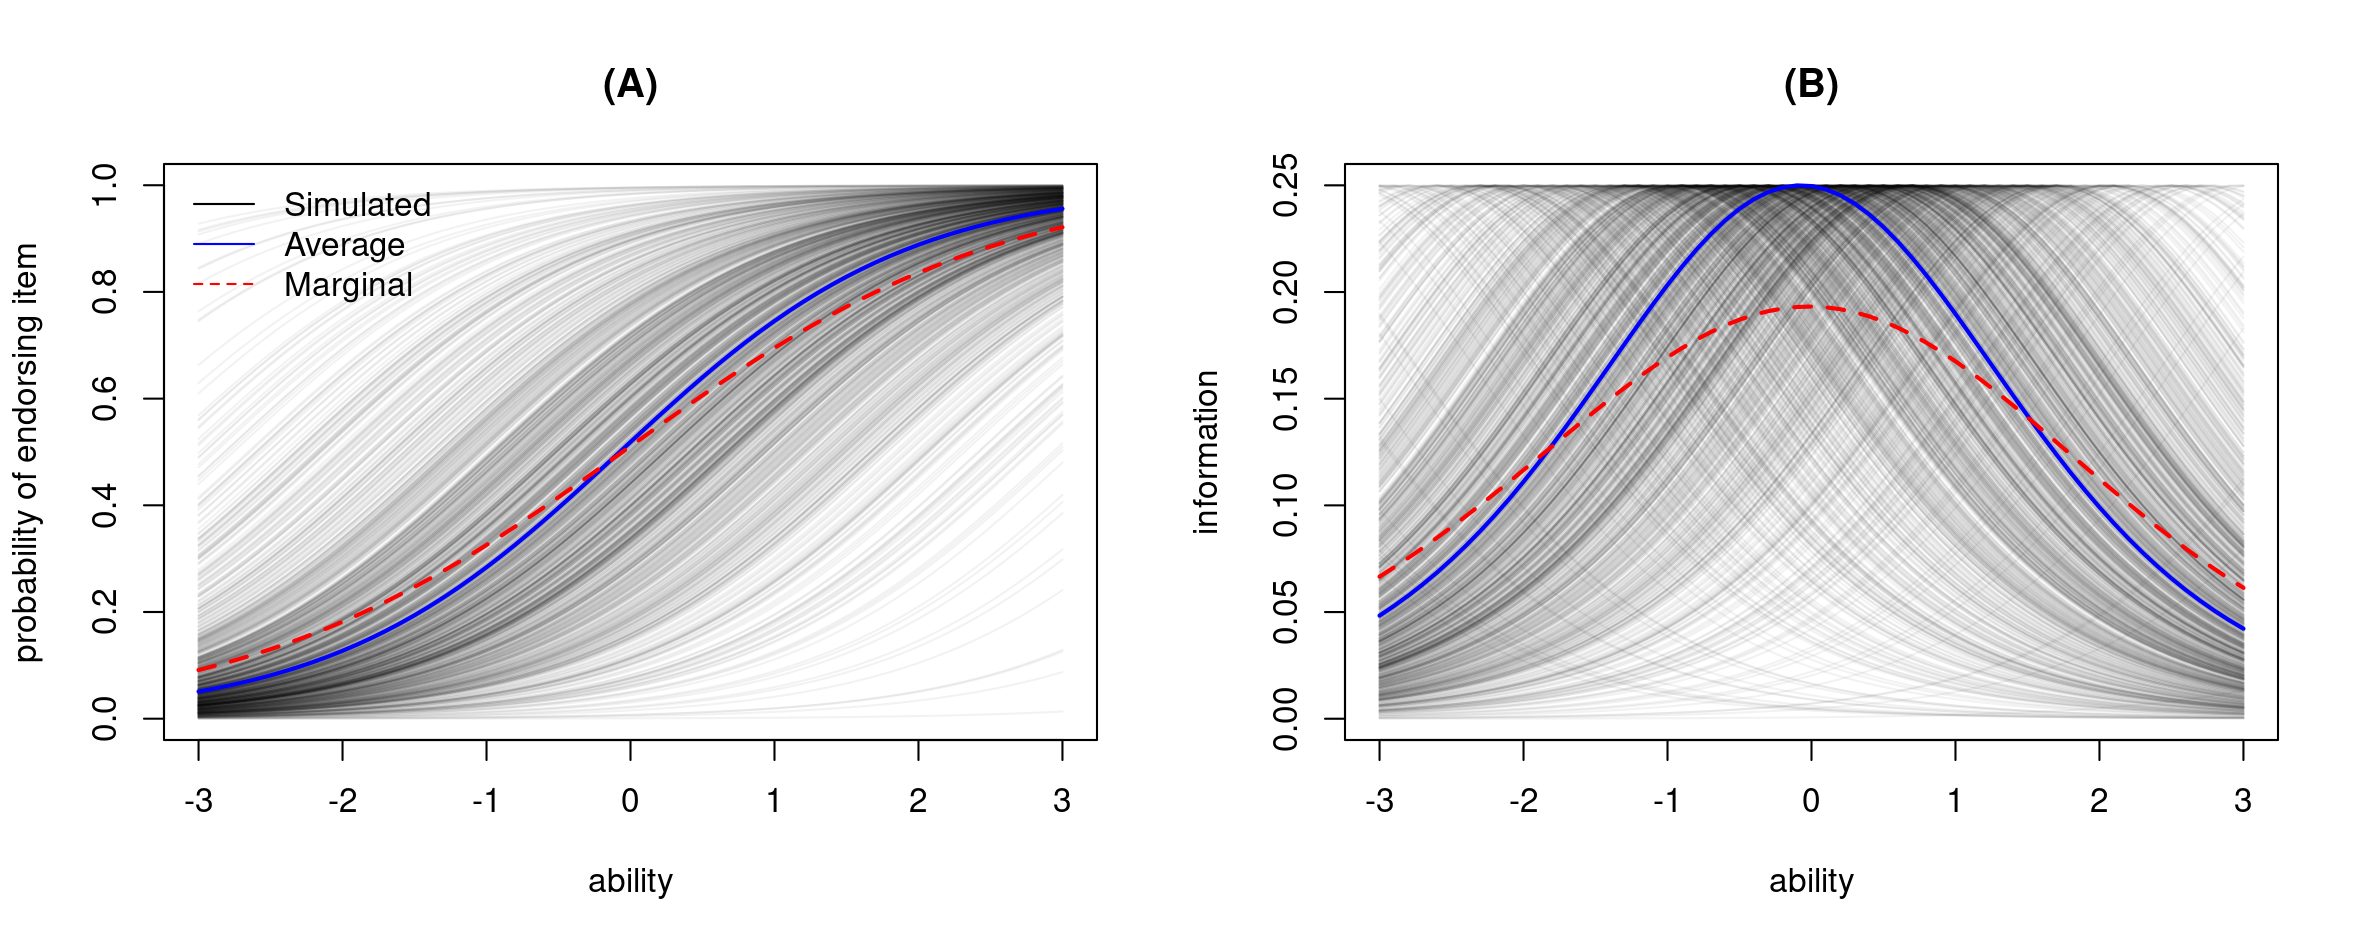
\includegraphics[width=1\linewidth]{SOLV_ICC_prior}
	%
	\caption[Second-Order latent variable model (SOLV). Item Characteristic Curve (ICC) and Item Information Function (IIF).]%
	{Second-Order latent variable model (SOLV). (A) Item Characteristics Curve, ICC. (B) Item Information Function, IIF.}
	\label{fig:SOLV_ICC_prior}
\end{figure}
%
\begin{figure}[H]
	\centering
	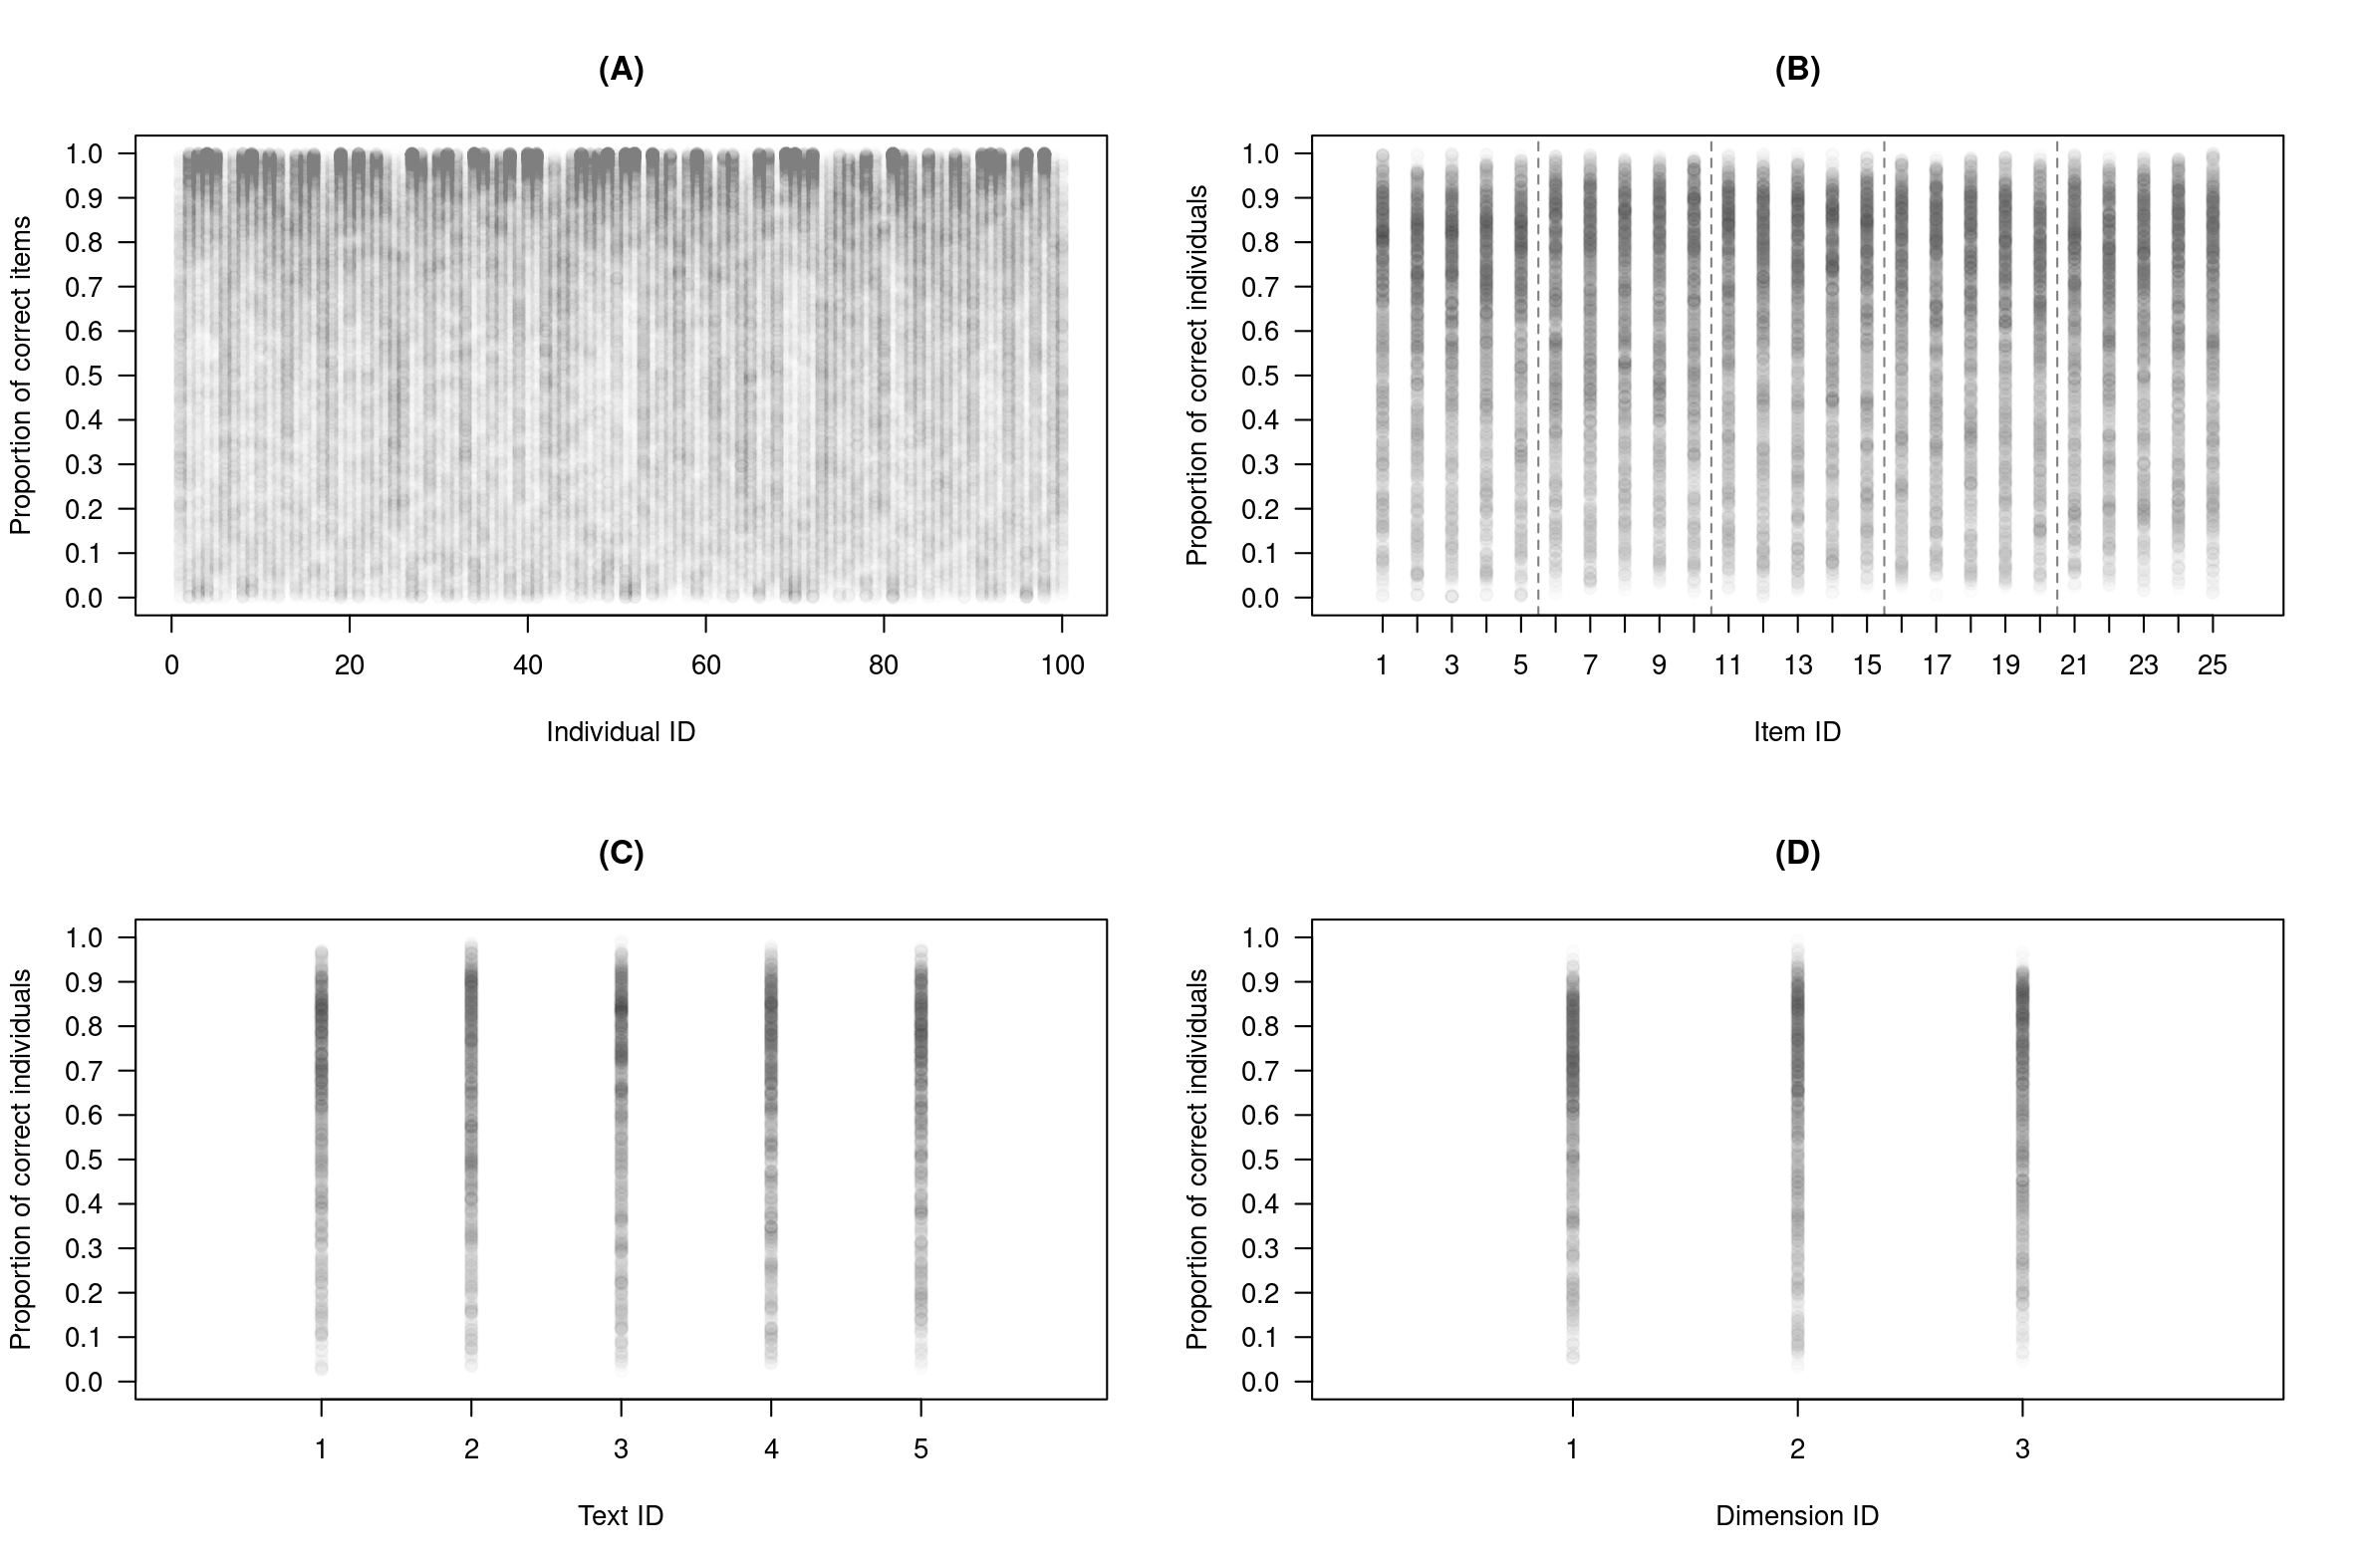
\includegraphics[width=1\linewidth]{SOLV_HitRate1}
	%
	\caption[Second-Order latent variable model (SOLV). Hit rate per dimensions of interest.]%
	{Second-Order latent variable model (SOLV). Aggregated endorsement rate per: (A) individuals, (B) items, (C) text or passage, and (D) measured dimension.}
	\label{fig:SOLV_hitrate1}
\end{figure}
%
\begin{figure}[H]
	\centering
	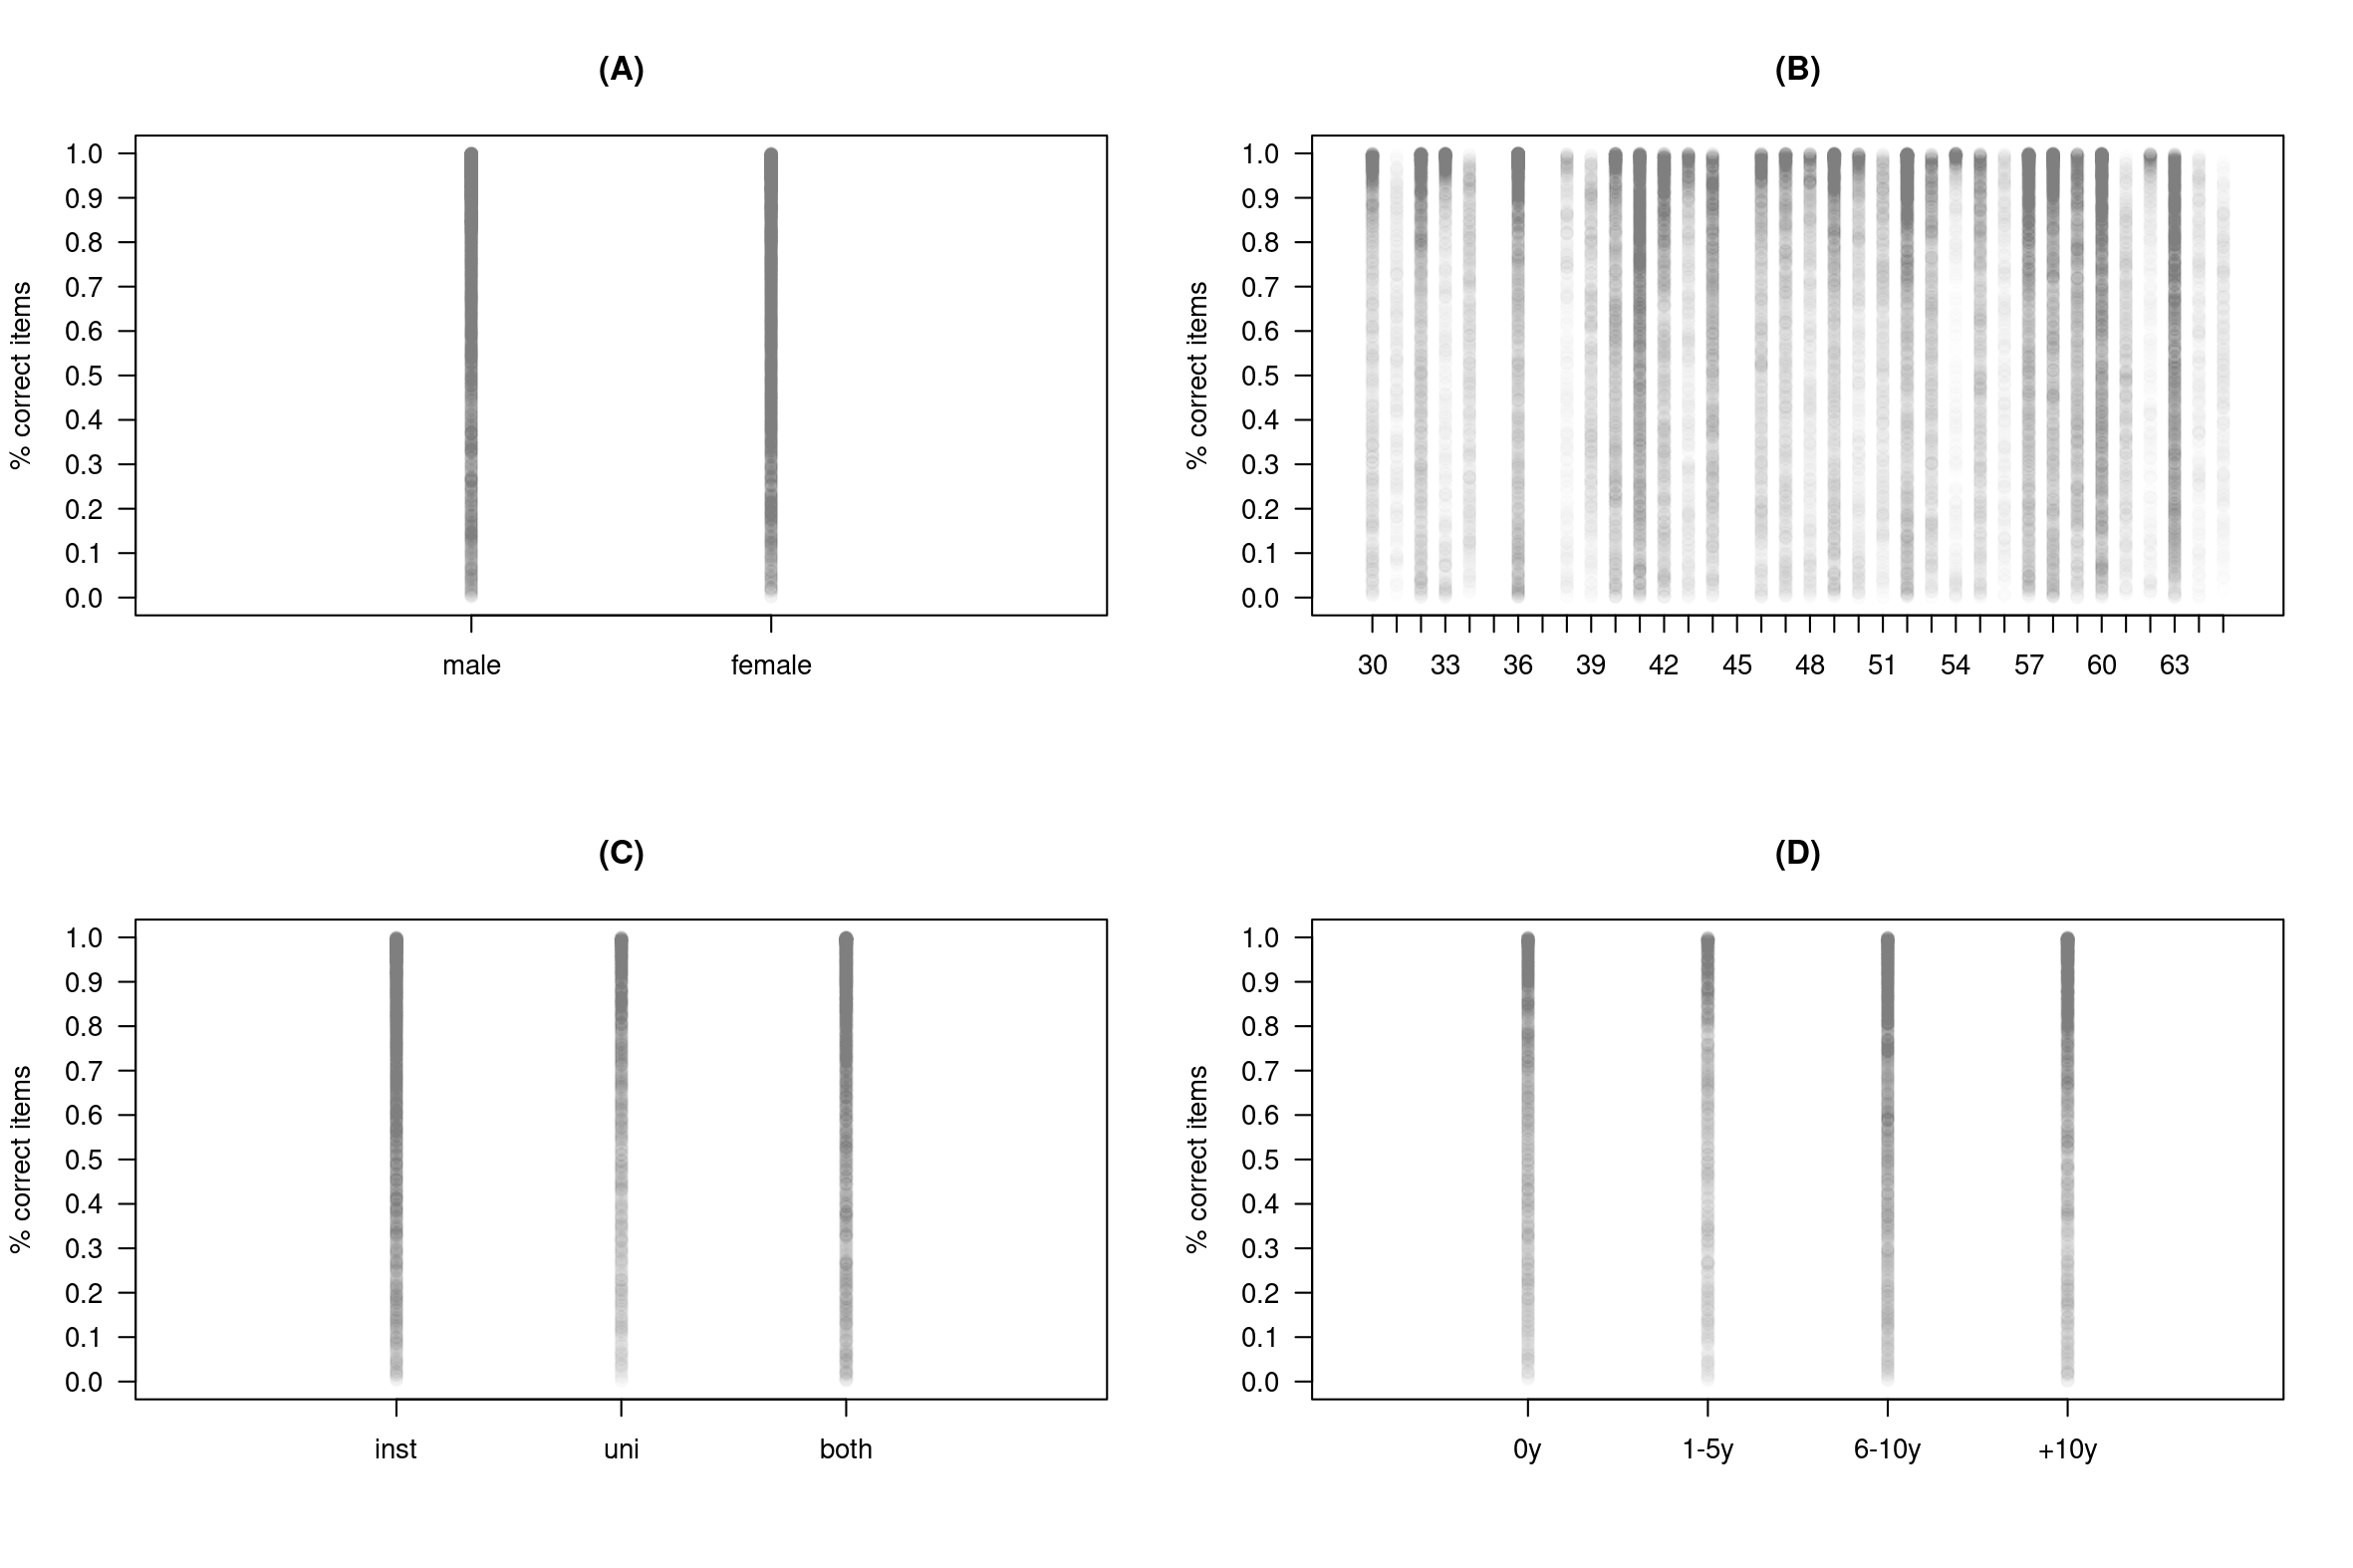
\includegraphics[width=1\linewidth]{SOLV_HitRate2}
	%
	\caption[Second-Order latent variable model (SOLV). Hit rate per simulated covariate.]%
	{Second-Order latent variable model (SOLV). Aggregated endorsement rate per simulated covariate: (A) gender, (B) age, (C) education, and (D) experience.}
	\label{fig:SOLV_hitrate2}
\end{figure}


\subsection{Chain performance}

Trace, trank and ACF plots for all models, parametrizations, and replicas can be found in the images section of the accompanying github page:

\noindent \url{https://github.com/jriveraespejo/thesis/tree/master/images/chains} \\

\noindent The CP and NCP comparison plots of effective sample sizes (\texttt{n\_eff}) and \texttt{Rhat}, for both models (across replicas), can be found in the corresponding image section of the accompanying github page:

\noindent \url{https://github.com/jriveraespejo/thesis/tree/master/images/chains_stat}
%
\begin{figure}[H]
	\centering
	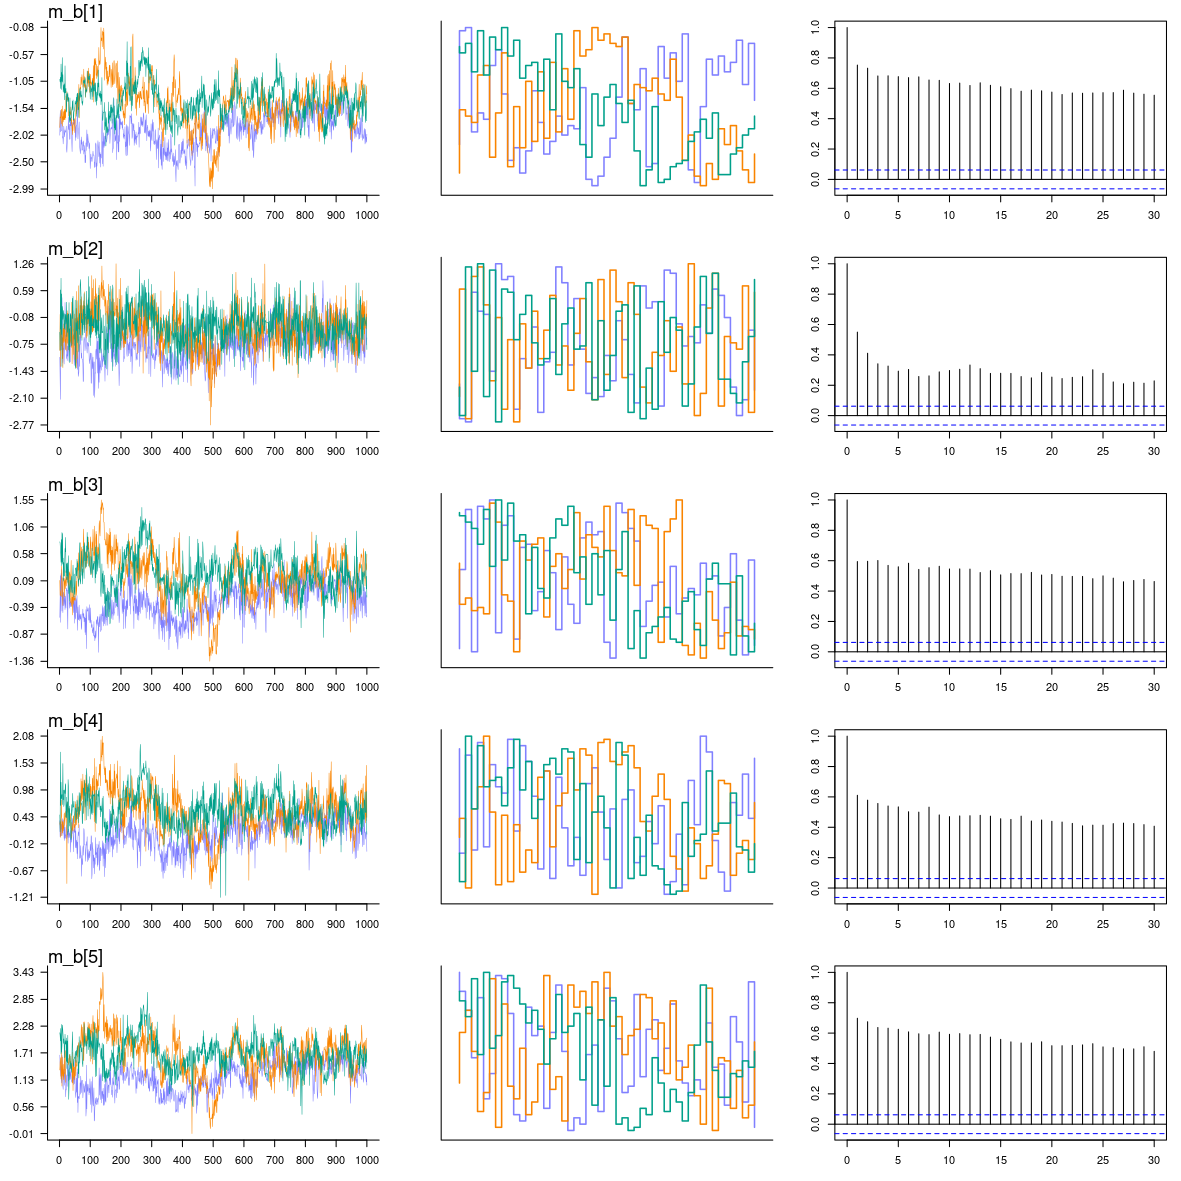
\includegraphics[width=1\linewidth]{FOLV_CE_J100_Ndata2_mb}
	%
	\caption[First-Order latent variable model (FOLV). Centered parametrization. Mean difficulty per text. Trace, trank and auto-correlation plots.]%
	{First-Order latent variable model (FOLV). Centered parametrization. Mean difficulty per text: (Left) trace plot, (Middle) trank plot, (Right) auto-correlation plot.}
	\label{fig:FOLV_CE_chains1}
\end{figure}
%
\begin{figure}[H]
	\centering
	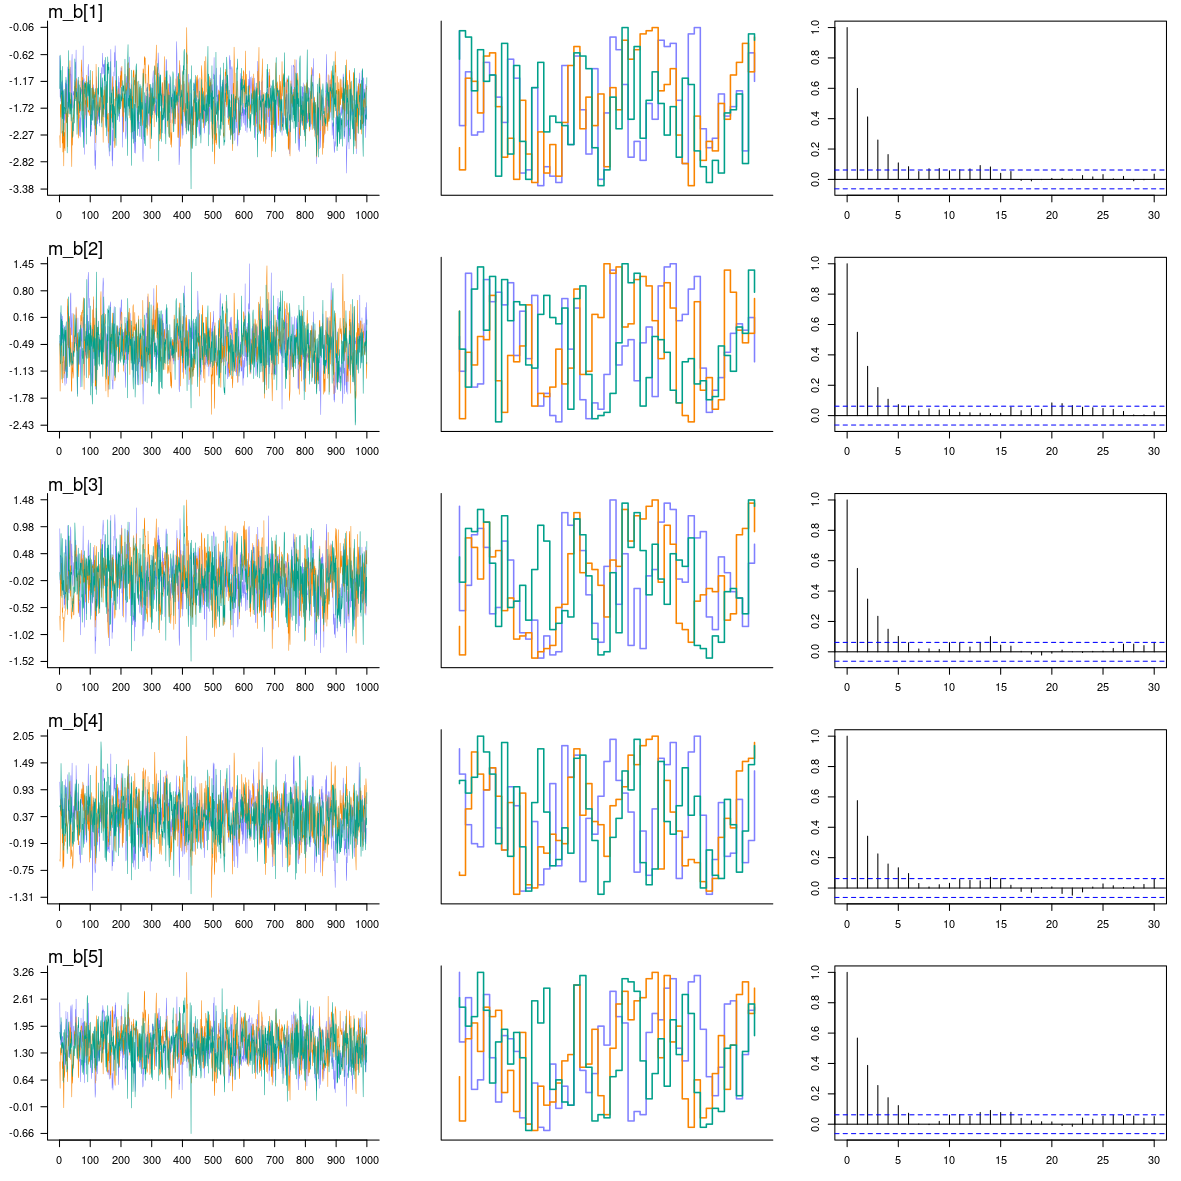
\includegraphics[width=1\linewidth]{FOLV_NC_J100_Ndata2_mb}
	%
	\caption[First-Order latent variable model (FOLV). Non-centered parametrization. Mean difficulty per text. Trace, trank and auto-correlation plots.]%
	{First-Order latent variable model (FOLV). Non-centered parametrization. Mean difficulty per text: (Left) trace plot, (Middle) trank plot, (Right) auto-correlation plot.}
	\label{fig:FOLV_NC_chains1}
\end{figure}
%
\begin{figure}[H]
	\centering
	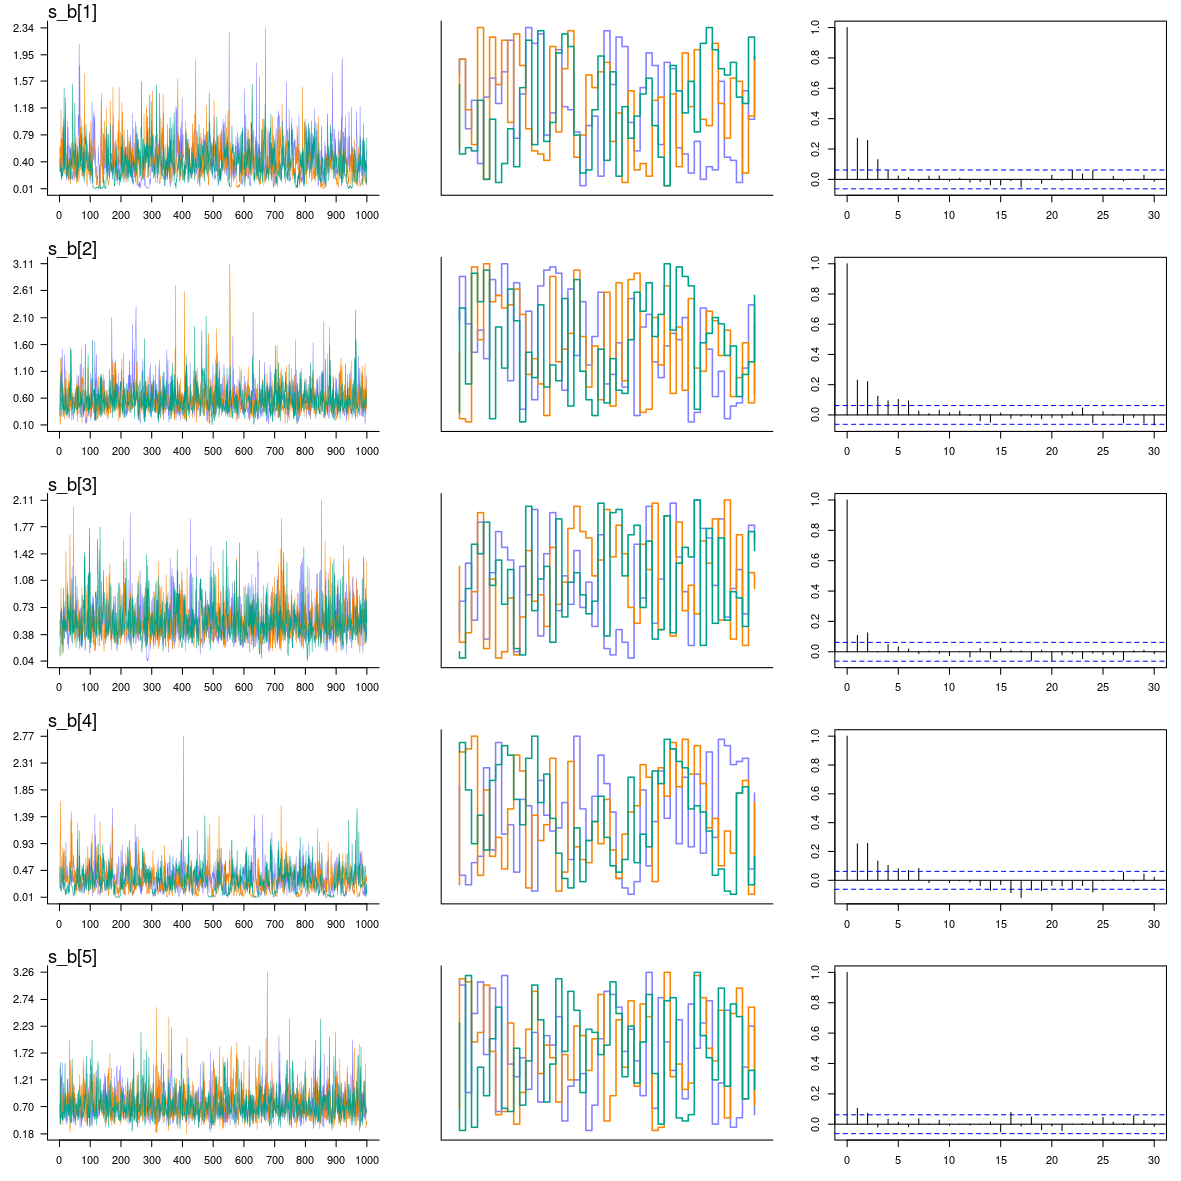
\includegraphics[width=1\linewidth]{FOLV_CE_J100_Ndata3_sb}
	%
	\caption[First-Order latent variable model (FOLV). Centered parametrization. Difficulty deviation per text. Trace, trank and auto-correlation plots.]%
	{First-Order latent variable model (FOLV). Centered parametrization. Difficulty deviation per text: (Left) trace plot, (Middle) trank plot, (Right) auto-correlation plot.}
	\label{fig:FOLV_CE_chains2}
\end{figure}
%
\begin{figure}[H]
	\centering
	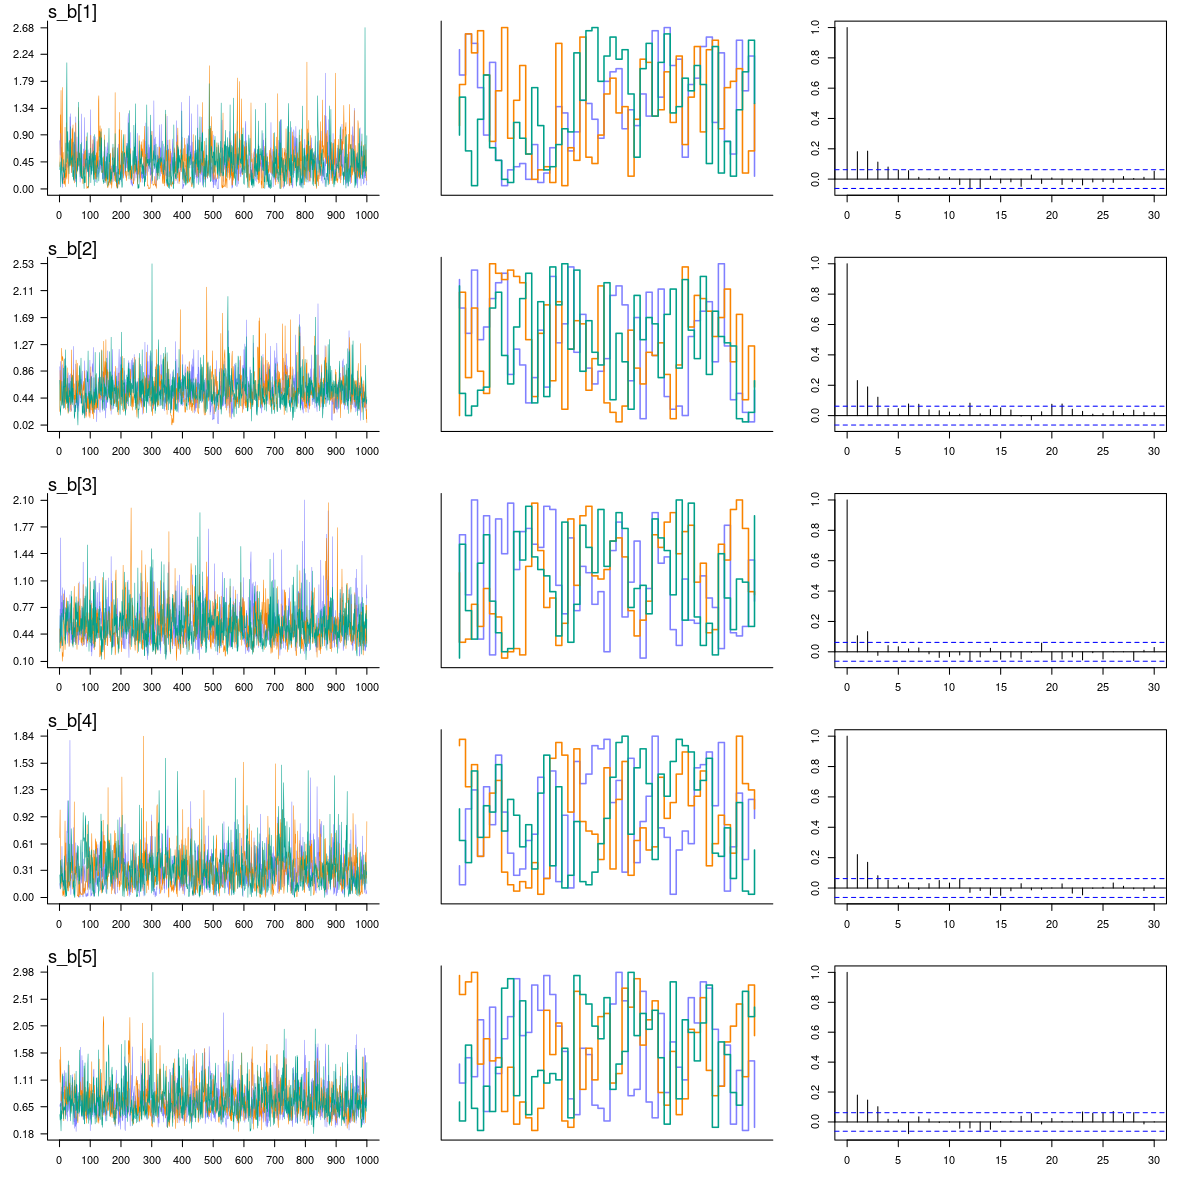
\includegraphics[width=1\linewidth]{FOLV_NC_J100_Ndata3_sb}
	%
	\caption[First-Order latent variable model (FOLV). Non-centered parametrization. Difficulty deviation per text. Trace, trank and auto-correlation plots.]%
	{First-Order latent variable model (FOLV). Non-centered parametrization. Difficulty deviation per text: (Left) trace plot, (Middle) trank plot, (Right) auto-correlation plot.}
	\label{fig:FOLV_NC_chains2}
\end{figure}
%
\begin{figure}[H]
	\centering
	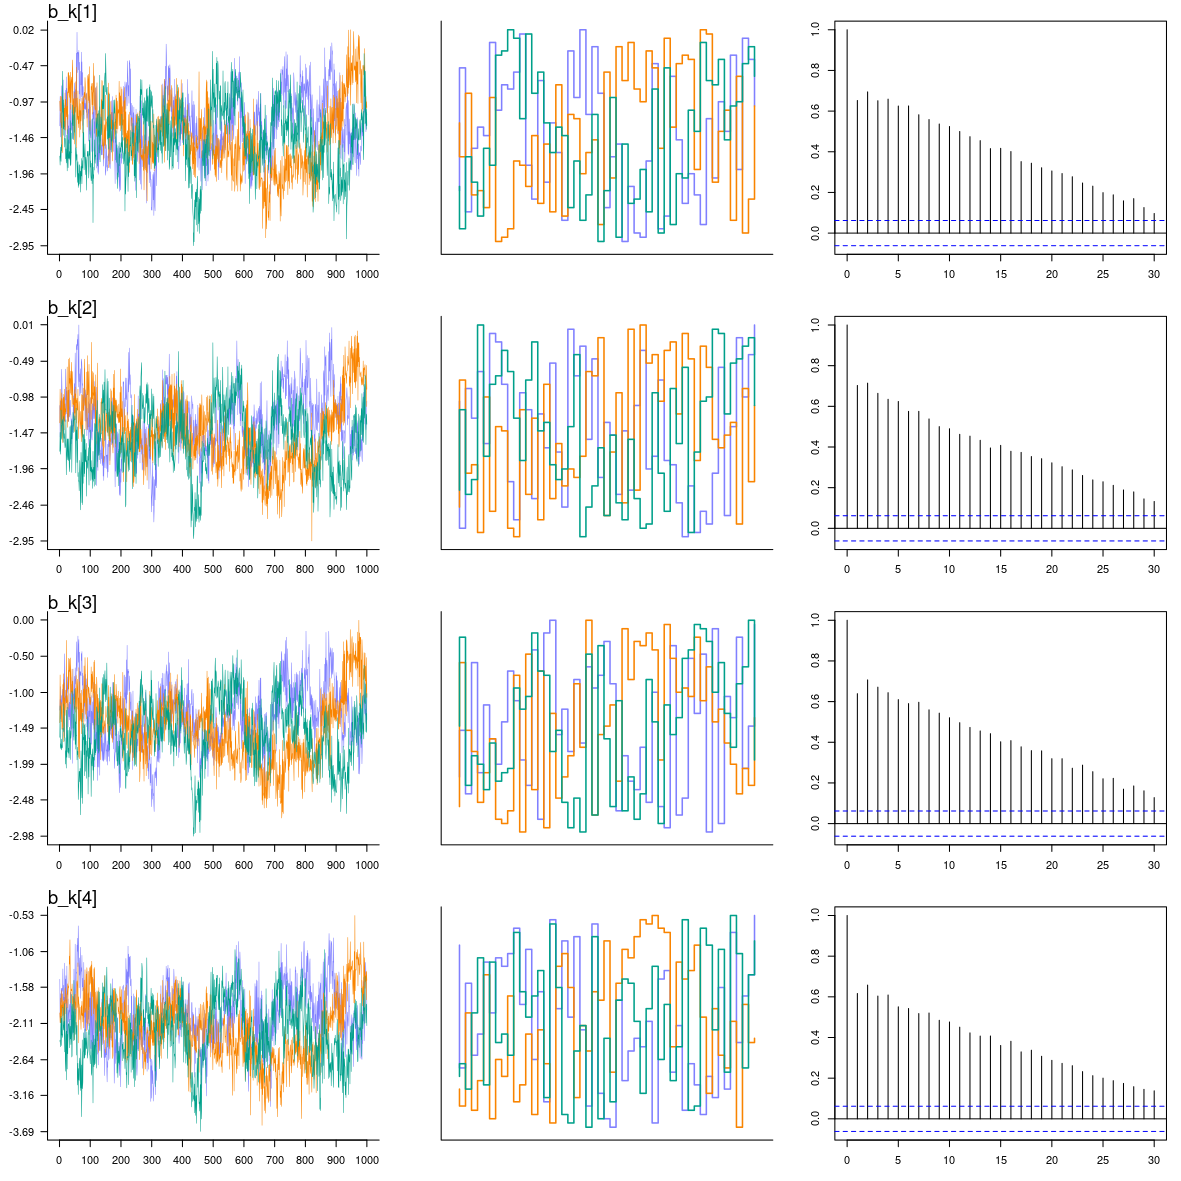
\includegraphics[width=1\linewidth]{FOLV_CE_J100_Ndata1_bk1}
	%
	\caption[First-Order latent variable model (FOLV). Centered parametrization. Difficulty per item. Trace, trank and auto-correlation plots.]%
	{First-Order latent variable model (FOLV). Centered parametrization. Difficulty per item: (Left) trace plot, (Middle) trank plot, (Right) auto-correlation plot.}
	\label{fig:FOLV_CE_chains3}
\end{figure}
%
\begin{figure}[H]
	\centering
	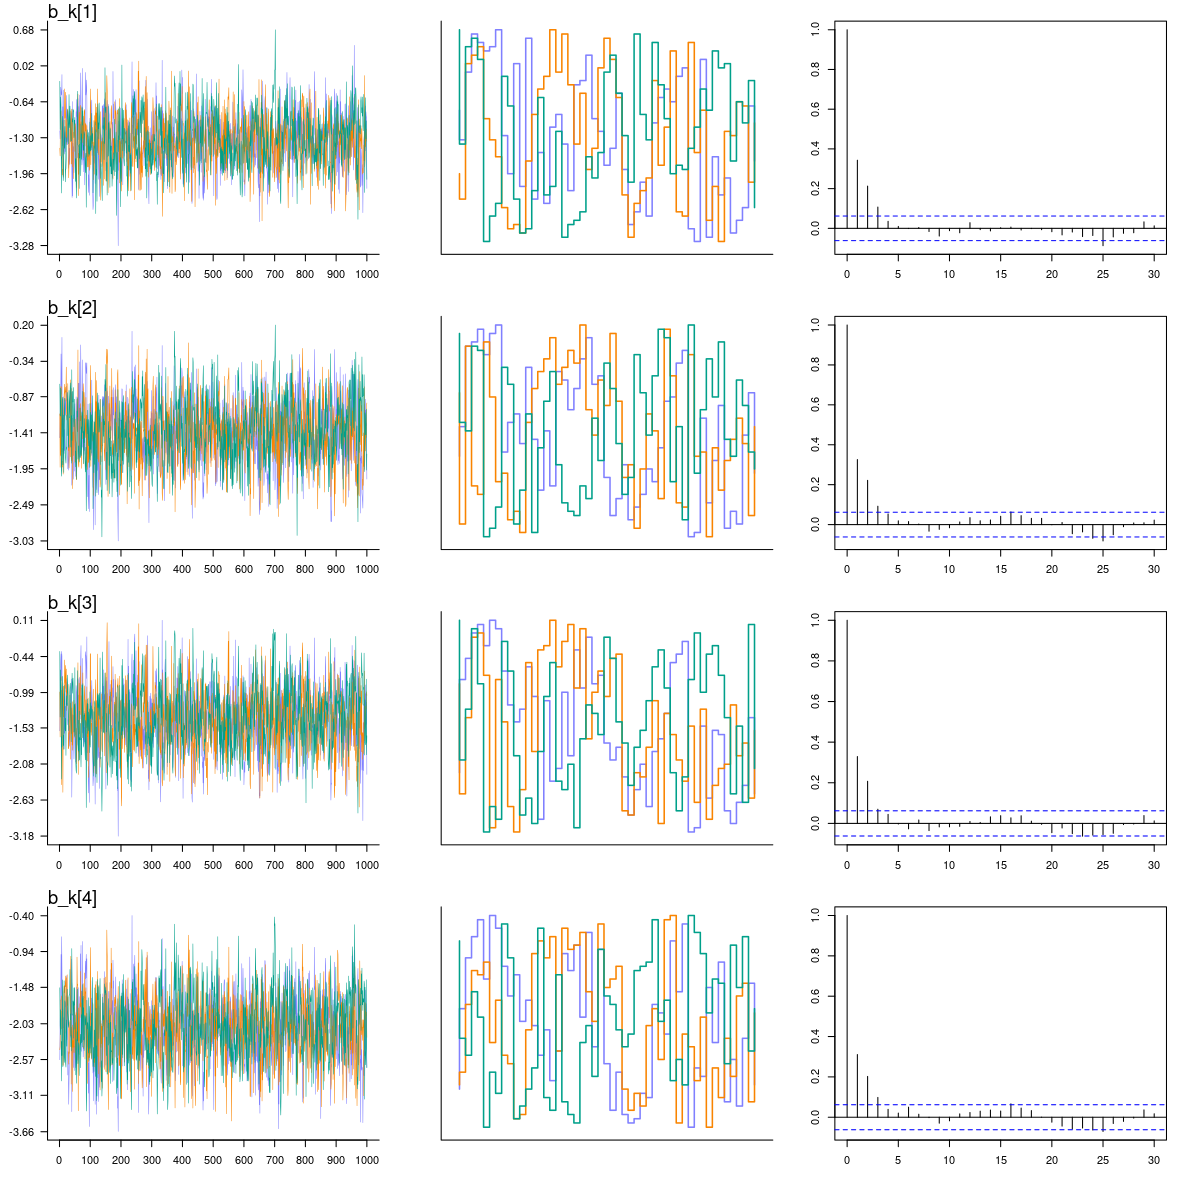
\includegraphics[width=1\linewidth]{FOLV_NC_J100_Ndata1_bk1}
	%
	\caption[First-Order latent variable model (FOLV). Non-centered parametrization. Difficulty per item. Trace, trank and auto-correlation plots.]%
	{First-Order latent variable model (FOLV). Non-centered parametrization. Difficulty per item: (Left) trace plot, (Middle) trank plot, (Right) auto-correlation plot.}
	\label{fig:FOLV_NC_chains3}
\end{figure}
%
\begin{figure}[H]
	\centering
	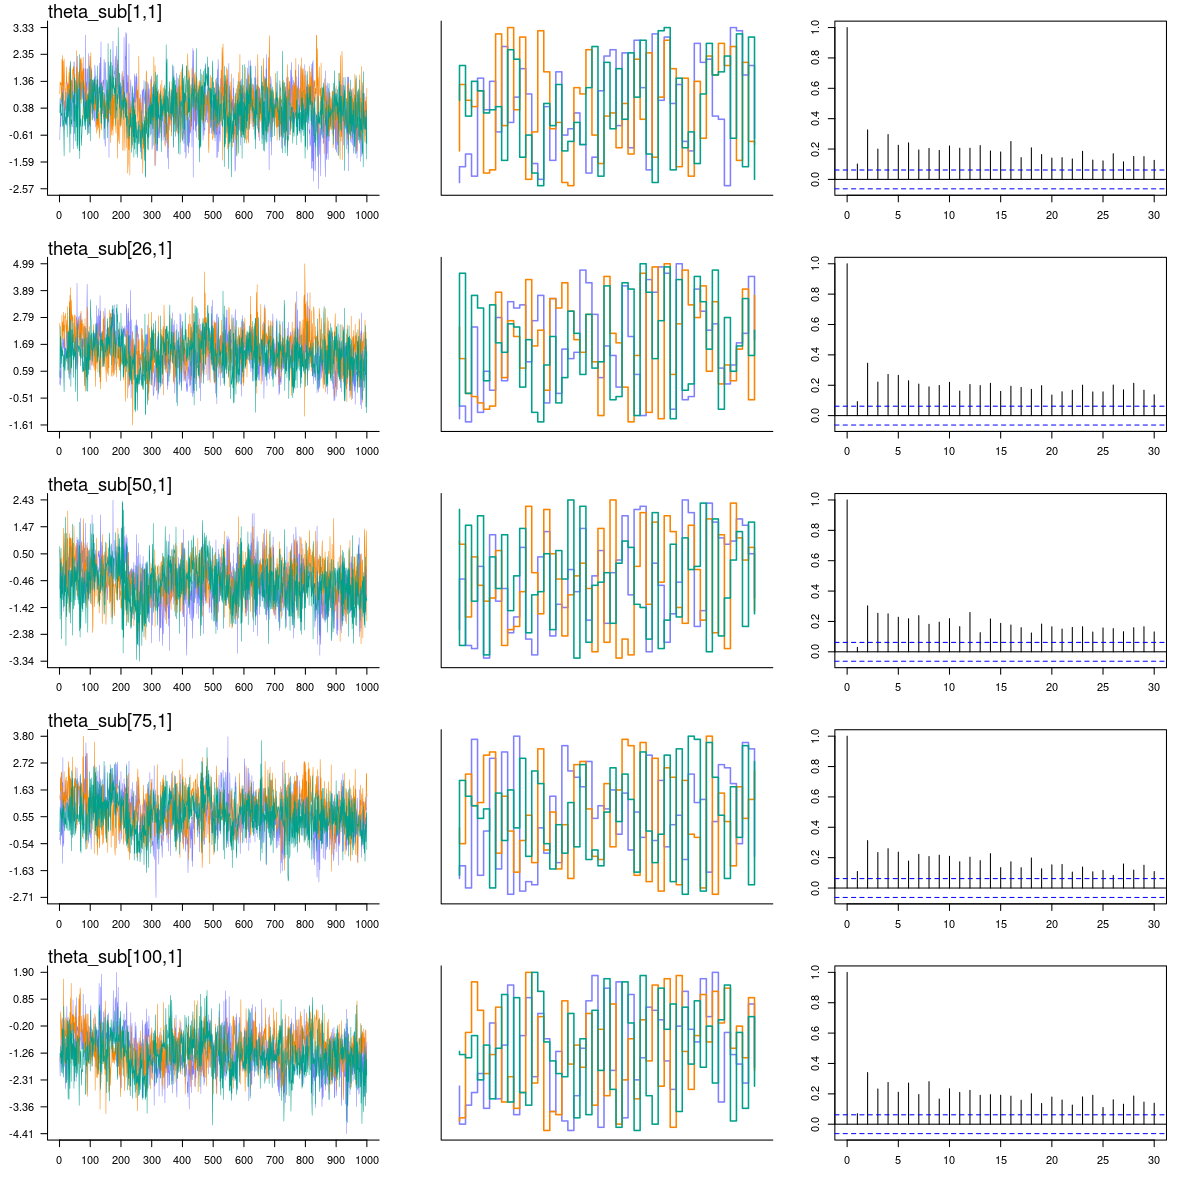
\includegraphics[width=1\linewidth]{FOLV_CE_J100_Ndata6_theta_sub1}
	%
	\caption[First-Order latent variable model (FOLV). Centered parametrization. Individual's first sub-dimension. Trace, trank and auto-correlation plots.]%
	{First-Order latent variable model (FOLV). Centered parametrization. Individual's first sub-dimension: (Left) trace plot, (Middle) trank plot, (Right) auto-correlation plot.}
	\label{fig:FOLV_CE_chains4}
\end{figure}
%
\begin{figure}[H]
	\centering
	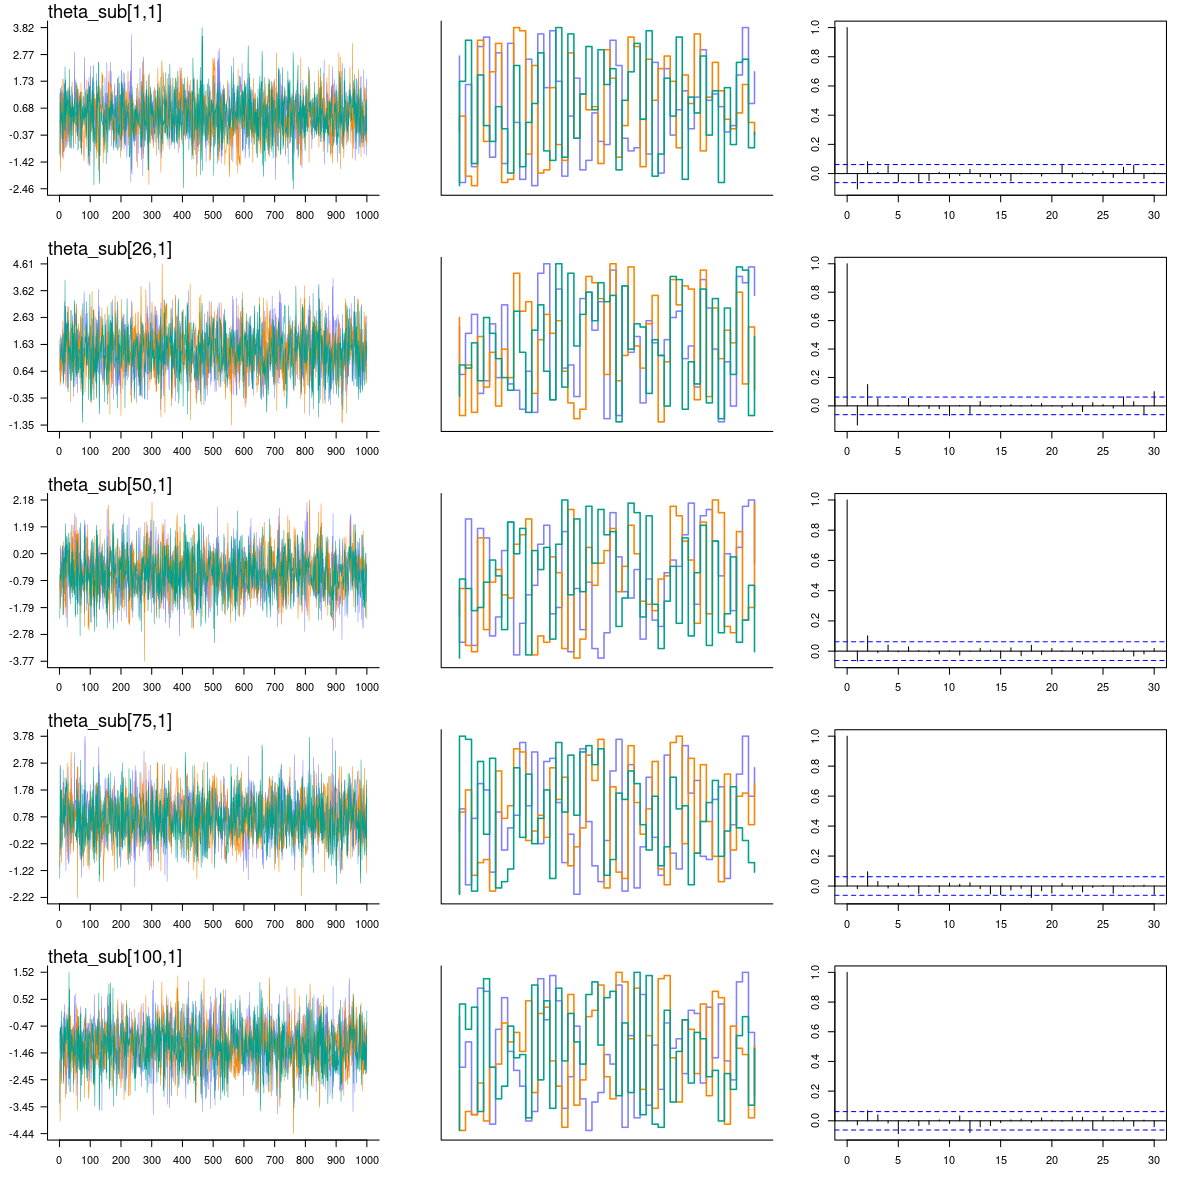
\includegraphics[width=1\linewidth]{FOLV_NC_J100_Ndata6_theta_sub1}
	%
	\caption[First-Order latent variable model (FOLV). Non-centered parametrization. Individual's first sub-dimension. Trace, trank and auto-correlation plots.]%
	{First-Order latent variable model (FOLV). Non-centered parametrization. Individual's first sub-dimension: (Left) trace plot, (Middle) trank plot, (Right) auto-correlation plot.}
	\label{fig:FOLV_NC_chains4}
\end{figure}
%
\begin{figure}[H]
	\centering
	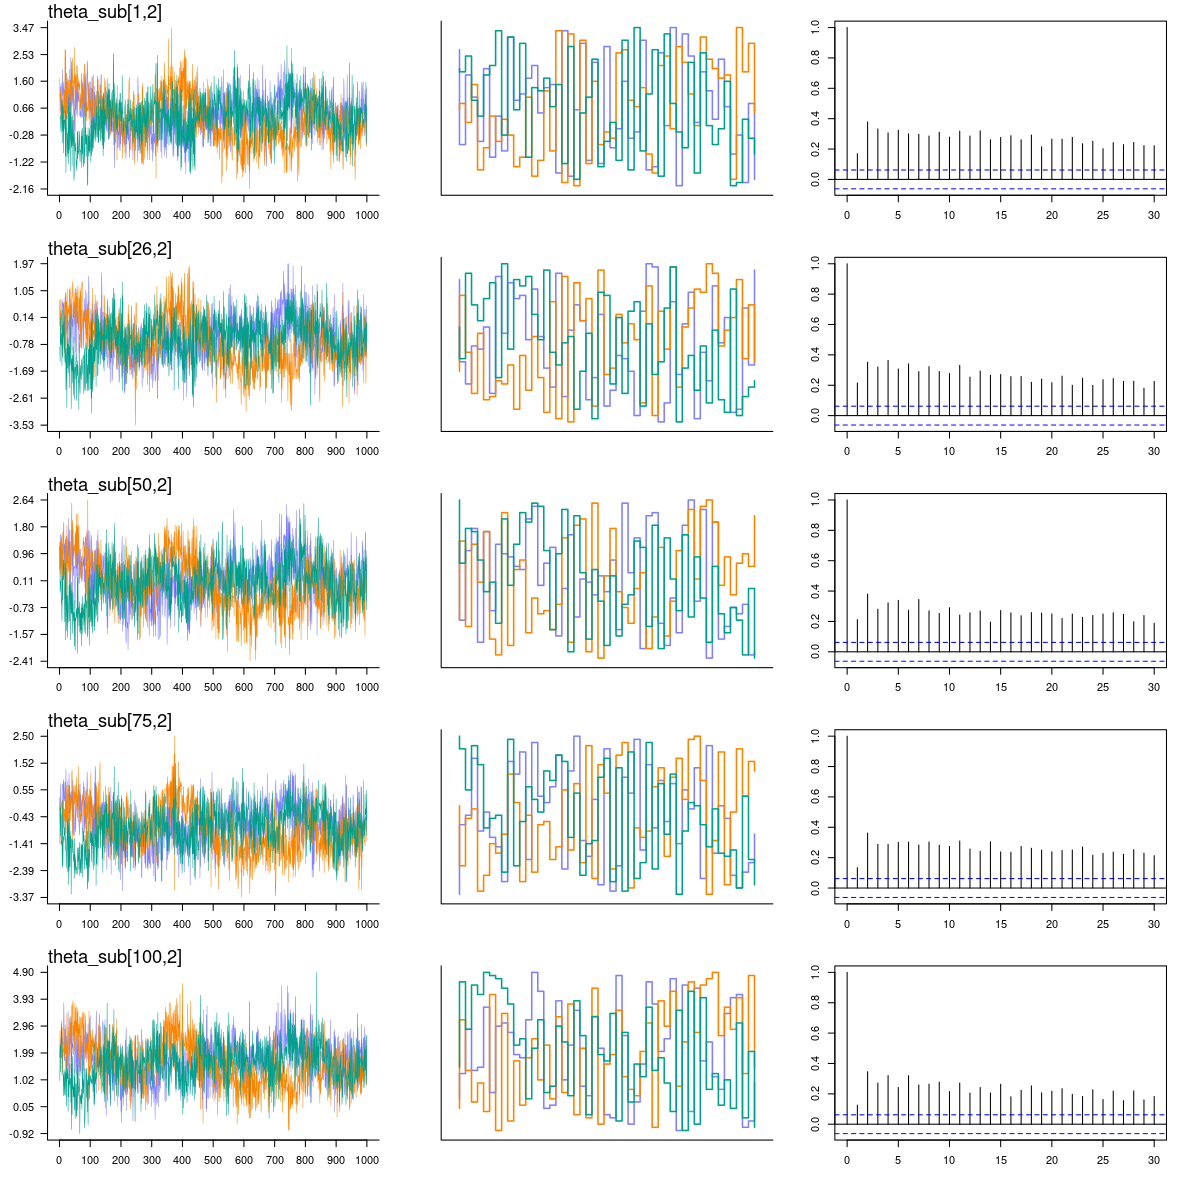
\includegraphics[width=1\linewidth]{FOLV_CE_J100_Ndata7_theta_sub2}
	%
	\caption[First-Order latent variable model (FOLV). Centered parametrization. Individual's second sub-dimension. Trace, trank and auto-correlation plots.]%
	{First-Order latent variable model (FOLV). Centered parametrization. Individual's second sub-dimension: (Left) trace plot, (Middle) trank plot, (Right) auto-correlation plot.}
	\label{fig:FOLV_CE_chains5}
\end{figure}
%
\begin{figure}[H]
	\centering
	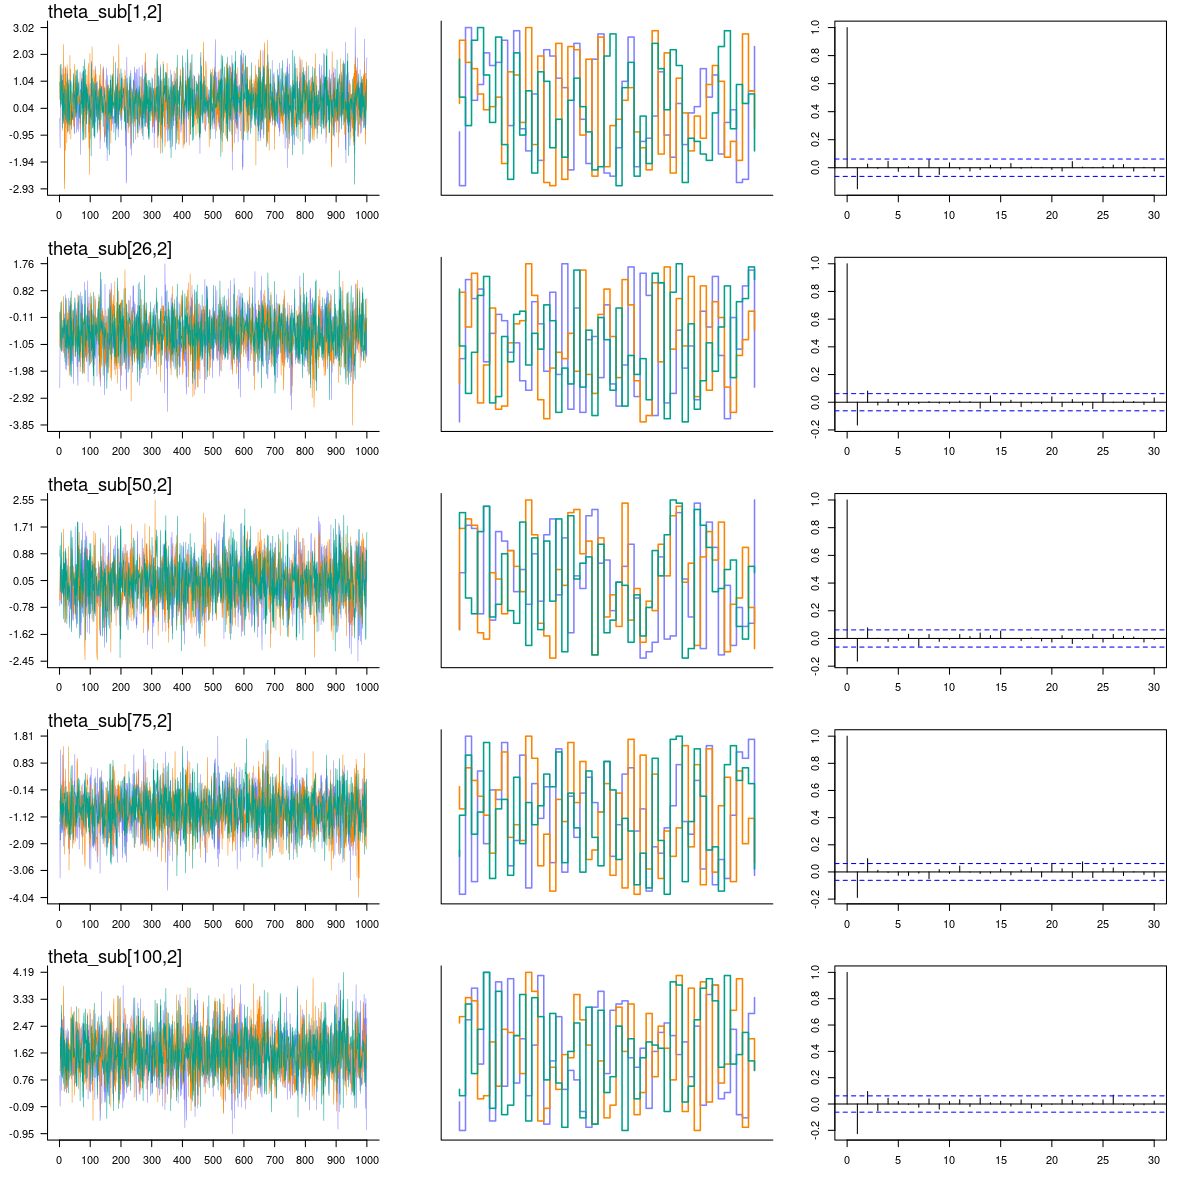
\includegraphics[width=1\linewidth]{FOLV_NC_J100_Ndata7_theta_sub2}
	%
	\caption[First-Order latent variable model (FOLV). Non-centered parametrization. Individual's second sub-dimension. Trace, trank and auto-correlation plots.]%
	{First-Order latent variable model (FOLV). Non-centered parametrization. Individual's second sub-dimension: (Left) trace plot, (Middle) trank plot, (Right) auto-correlation plot.}
	\label{fig:FOLV_NC_chains5}
\end{figure}
%
\begin{figure}[H]
	\centering
	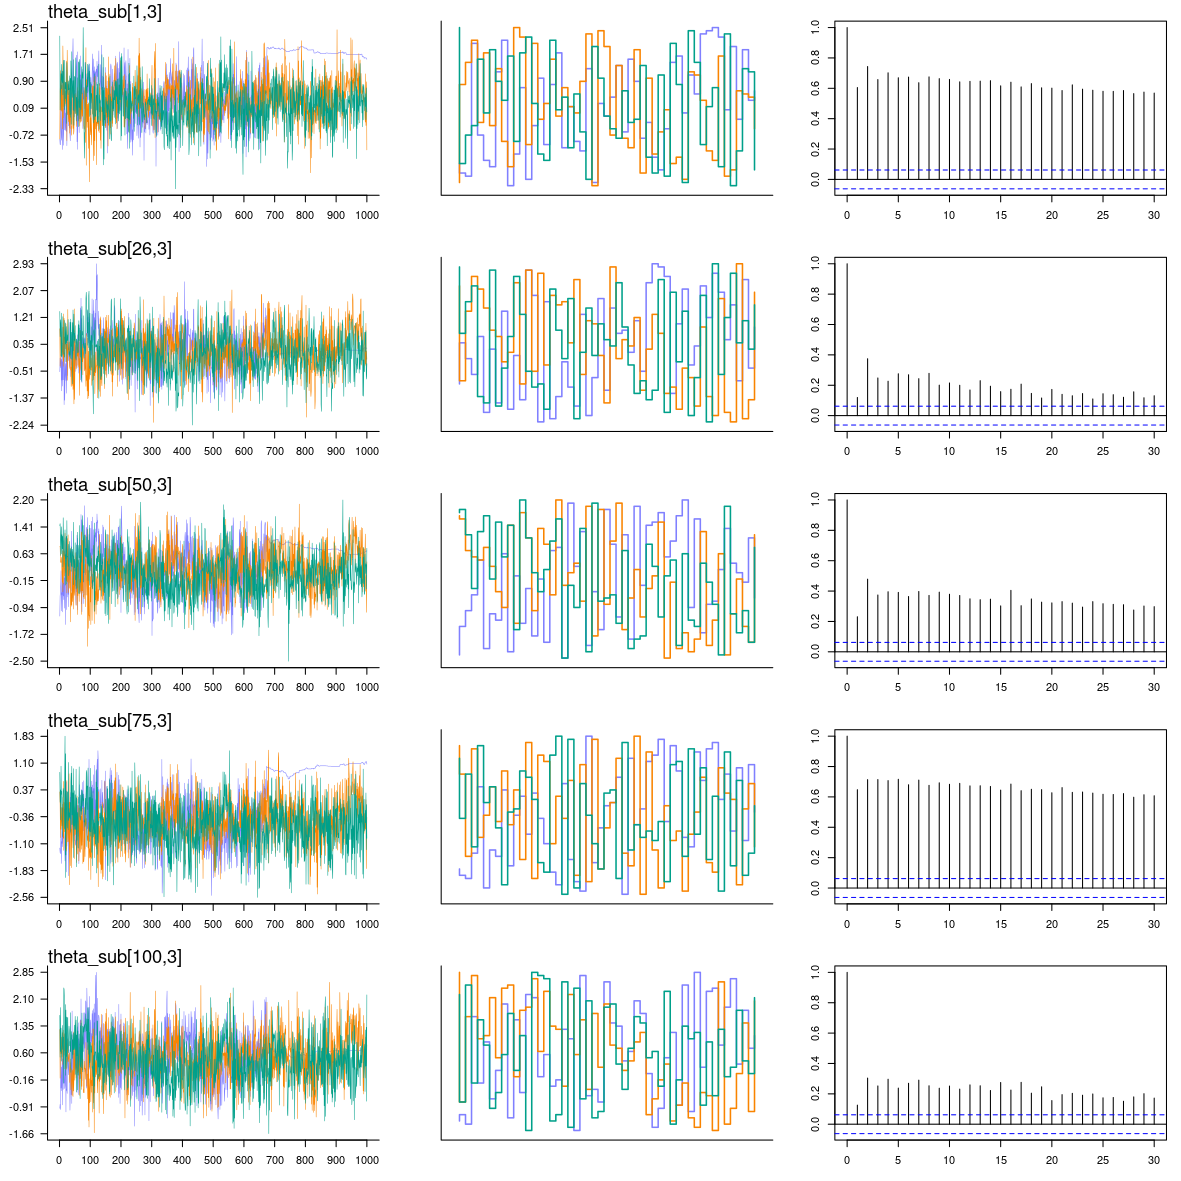
\includegraphics[width=1\linewidth]{FOLV_CE_J100_Ndata8_theta_sub3}
	%
	\caption[First-Order latent variable model (FOLV). Centered parametrization. Individual's third sub-dimension. Trace, trank and auto-correlation plots.]%
	{First-Order latent variable model (FOLV). Centered parametrization. Individual's third sub-dimension: (Left) trace plot, (Middle) trank plot, (Right) auto-correlation plot.}
	\label{fig:FOLV_CE_chains6}
\end{figure}
%
\begin{figure}[H]
	\centering
	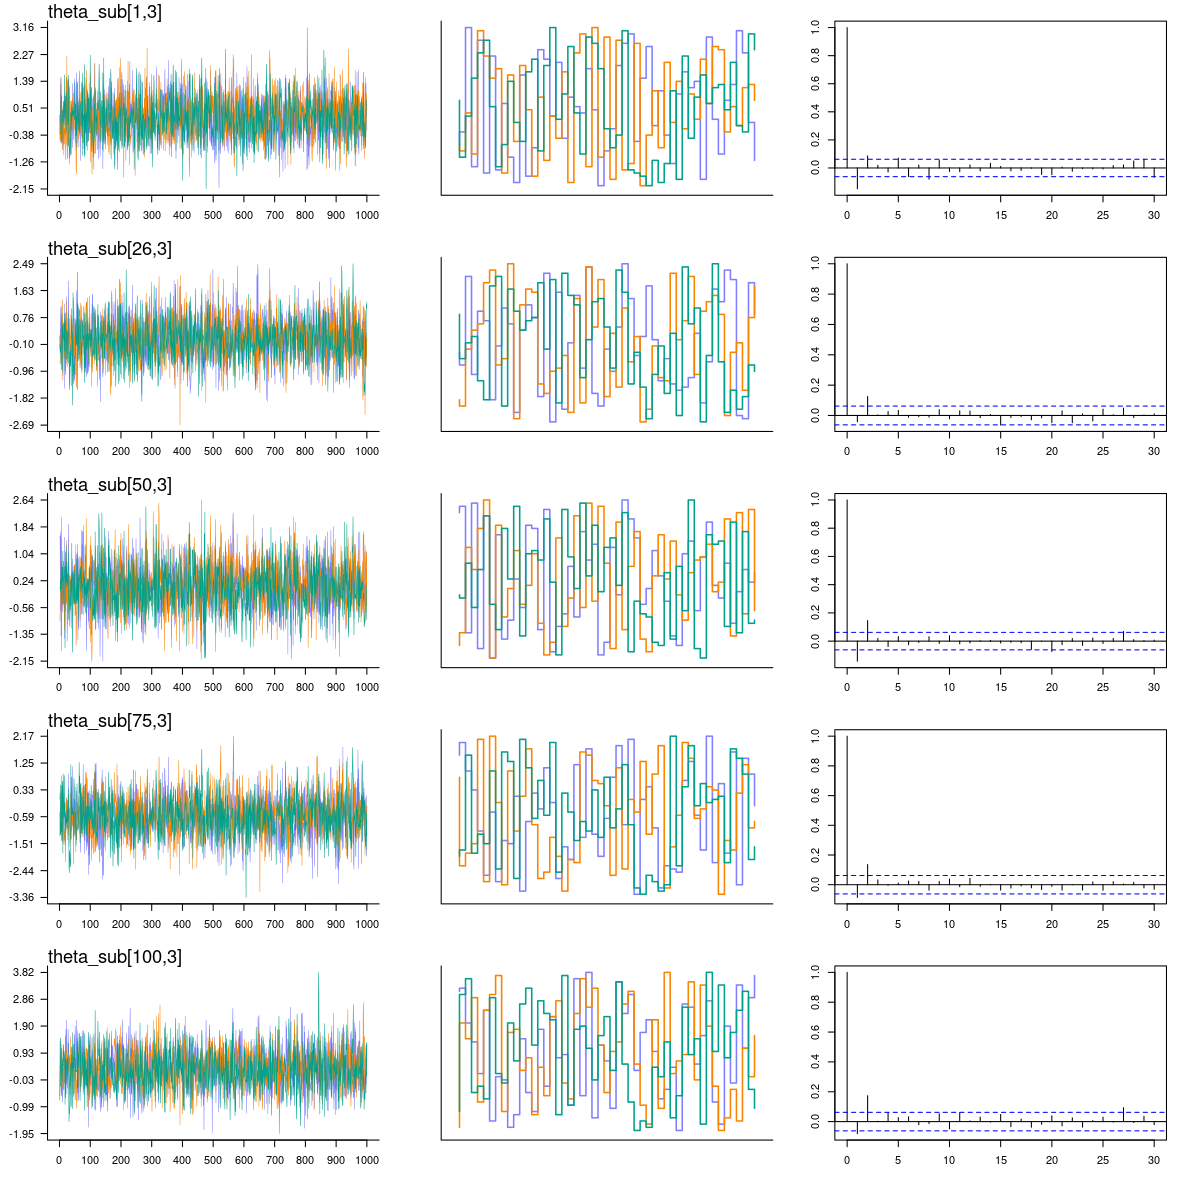
\includegraphics[width=1\linewidth]{FOLV_NC_J100_Ndata8_theta_sub3}
	%
	\caption[First-Order latent variable model (FOLV). Non-centered parametrization. Individual's third sub-dimension. Trace, trank and auto-correlation plots.]%
	{First-Order latent variable model (FOLV). Non-centered parametrization. Individual's third sub-dimension: (Left) trace plot, (Middle) trank plot, (Right) auto-correlation plot.}
	\label{fig:FOLV_NC_chains6}
\end{figure}
%
\begin{figure}[H]
	\centering
	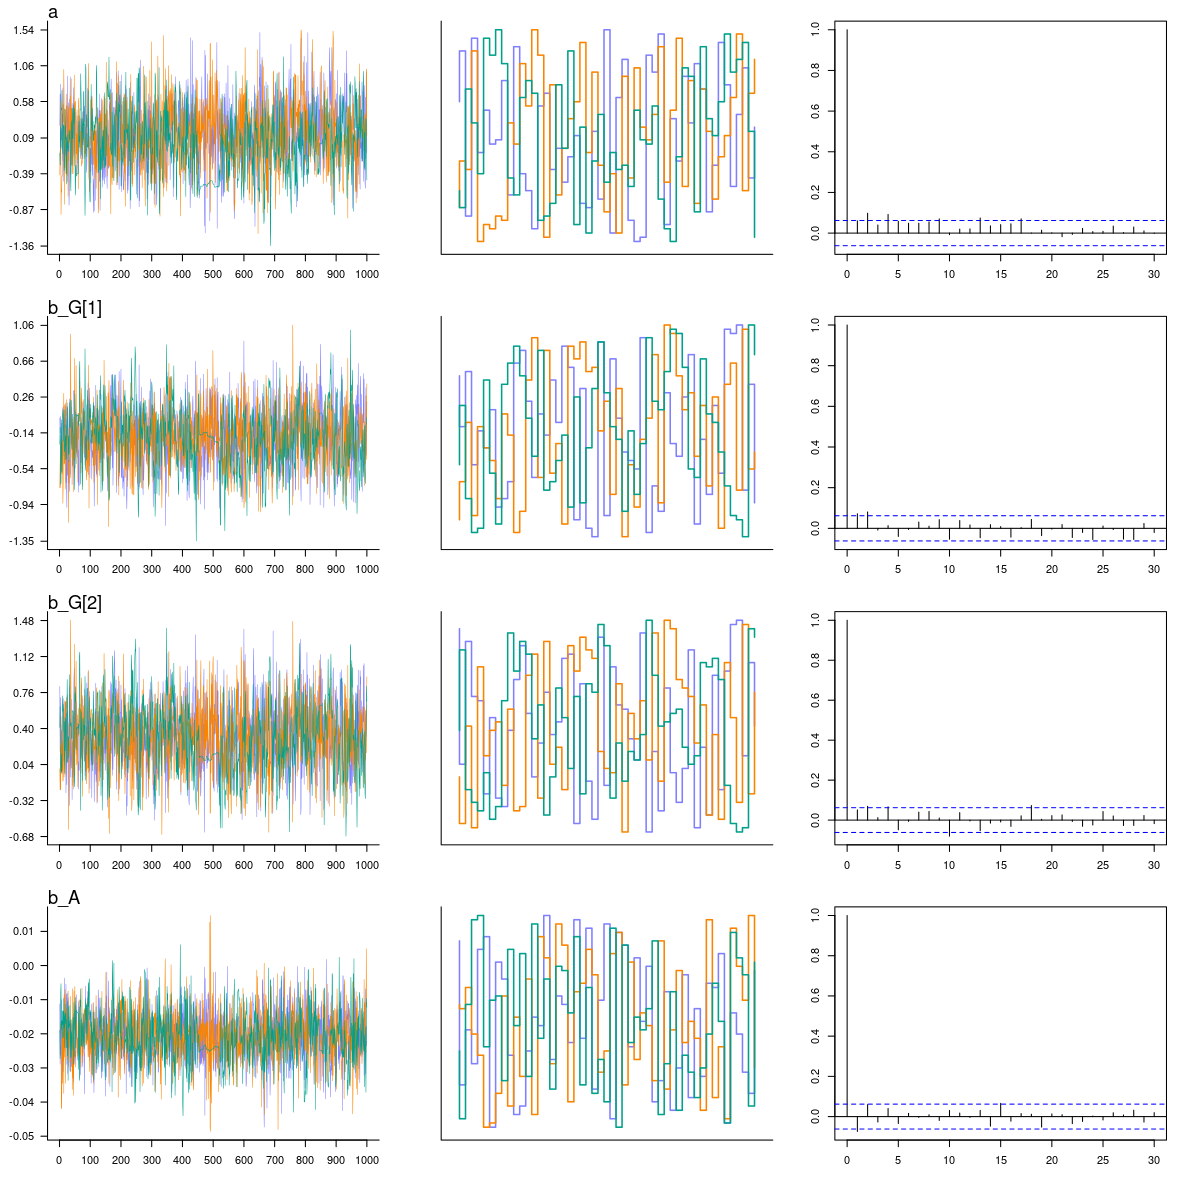
\includegraphics[width=1\linewidth]{FOLV_CE_J100_Ndata4_reg1}
	%
	\caption[First-Order latent variable model (FOLV). Centered parametrization. Regression parameters. Trace, trank and auto-correlation plots.]%
	{First-Order latent variable model (FOLV). Centered parametrization. Regression parameters: (Left) trace plot, (Middle) trank plot, (Right) auto-correlation plot.}
	\label{fig:FOLV_CE_chains7}
\end{figure}
%
\begin{figure}[H]
	\centering
	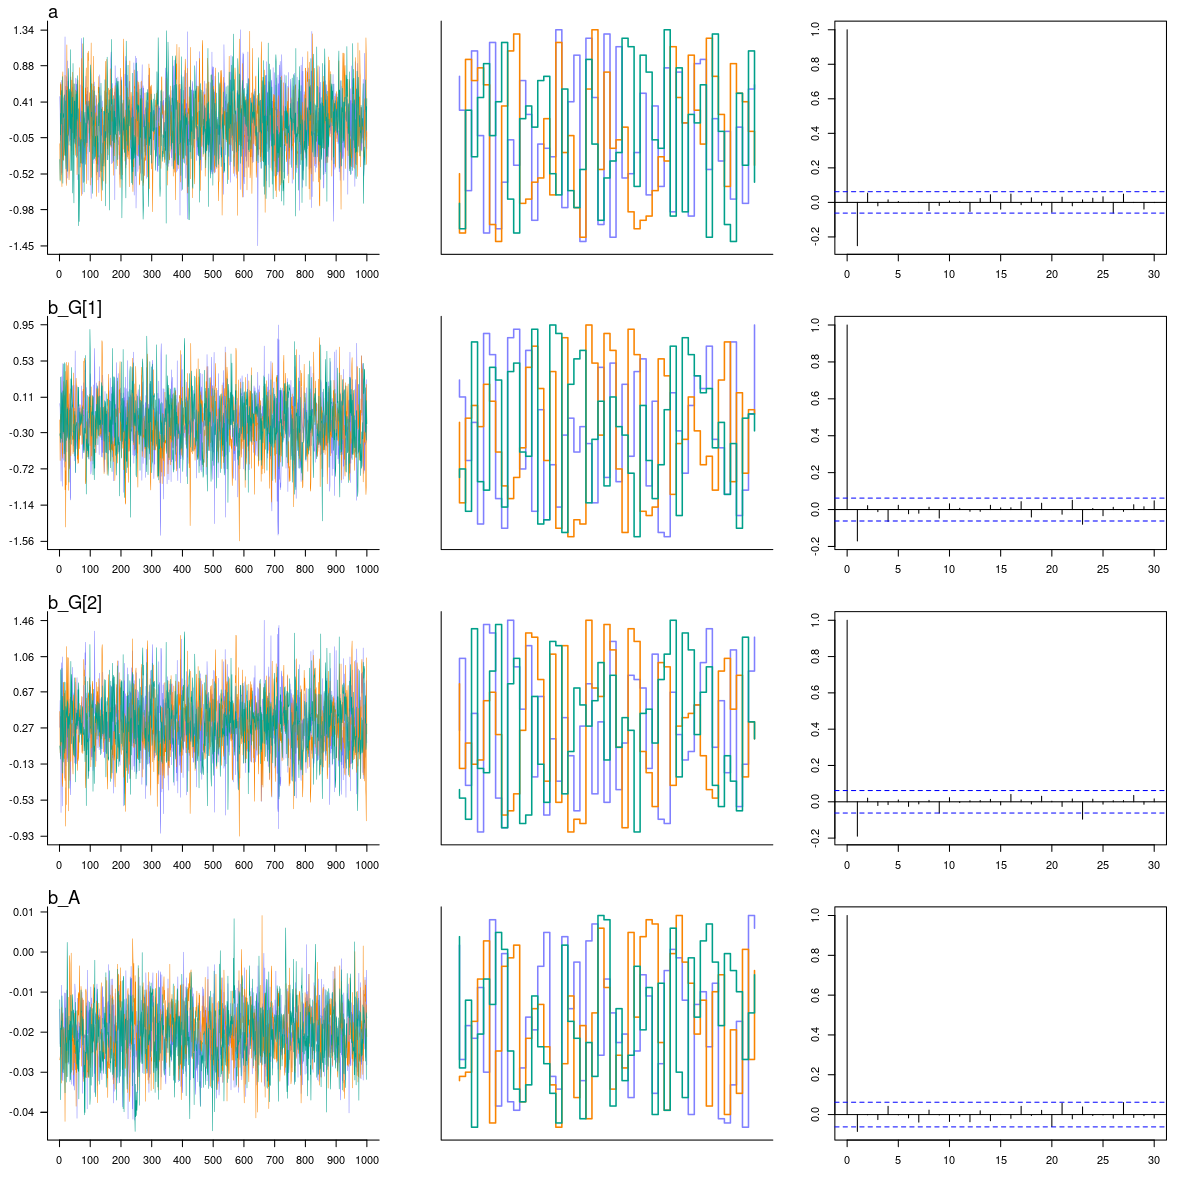
\includegraphics[width=1\linewidth]{FOLV_NC_J100_Ndata4_reg1}
	%
	\caption[First-Order latent variable model (FOLV). Non-centered parametrization. Regression parameters. Trace, trank and auto-correlation plots.]%
	{First-Order latent variable model (FOLV). Non-centered parametrization. Regression parameters: (Left) trace plot, (Middle) trank plot, (Right) auto-correlation plot.}
	\label{fig:FOLV_NC_chains7}
\end{figure}
%
\begin{figure}[H]
	\centering
	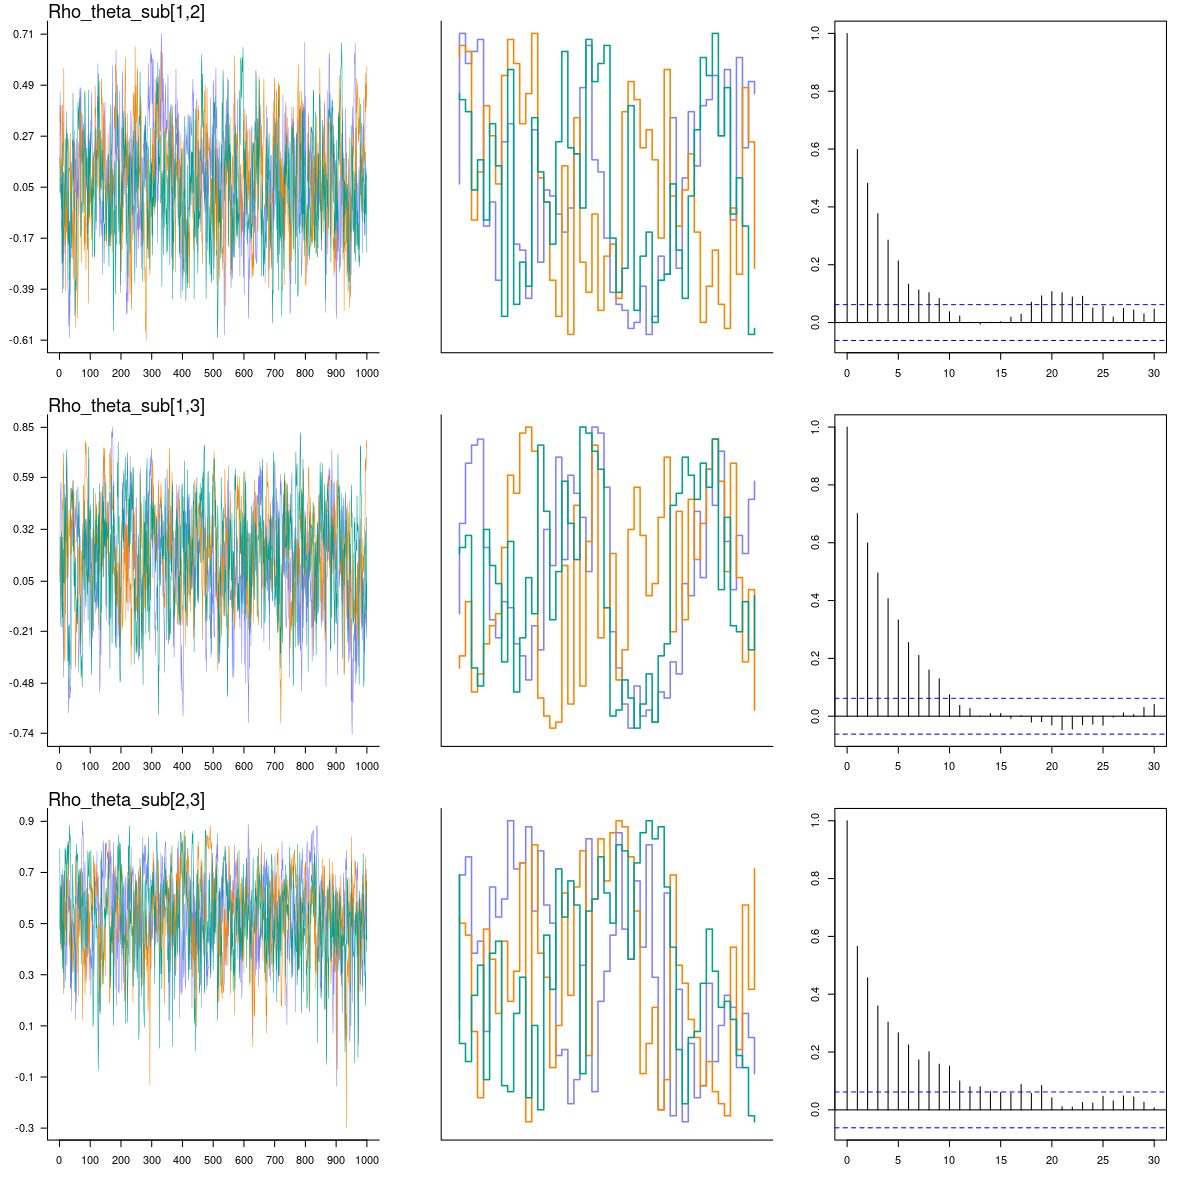
\includegraphics[width=1\linewidth]{FOLV_CE_J100_Ndata5_Rho}
	%
	\caption[First-Order latent variable model (FOLV). Centered parametrization. Correlation of sub-dimensions. Trace, trank and auto-correlation plots.]%
	{First-Order latent variable model (FOLV). Centered parametrization. Correlation of sub-dimensions: (Left) trace plot, (Middle) trank plot, (Right) auto-correlation plot.}
	\label{fig:FOLV_CE_chains8}
\end{figure}
%
\begin{figure}[H]
	\centering
	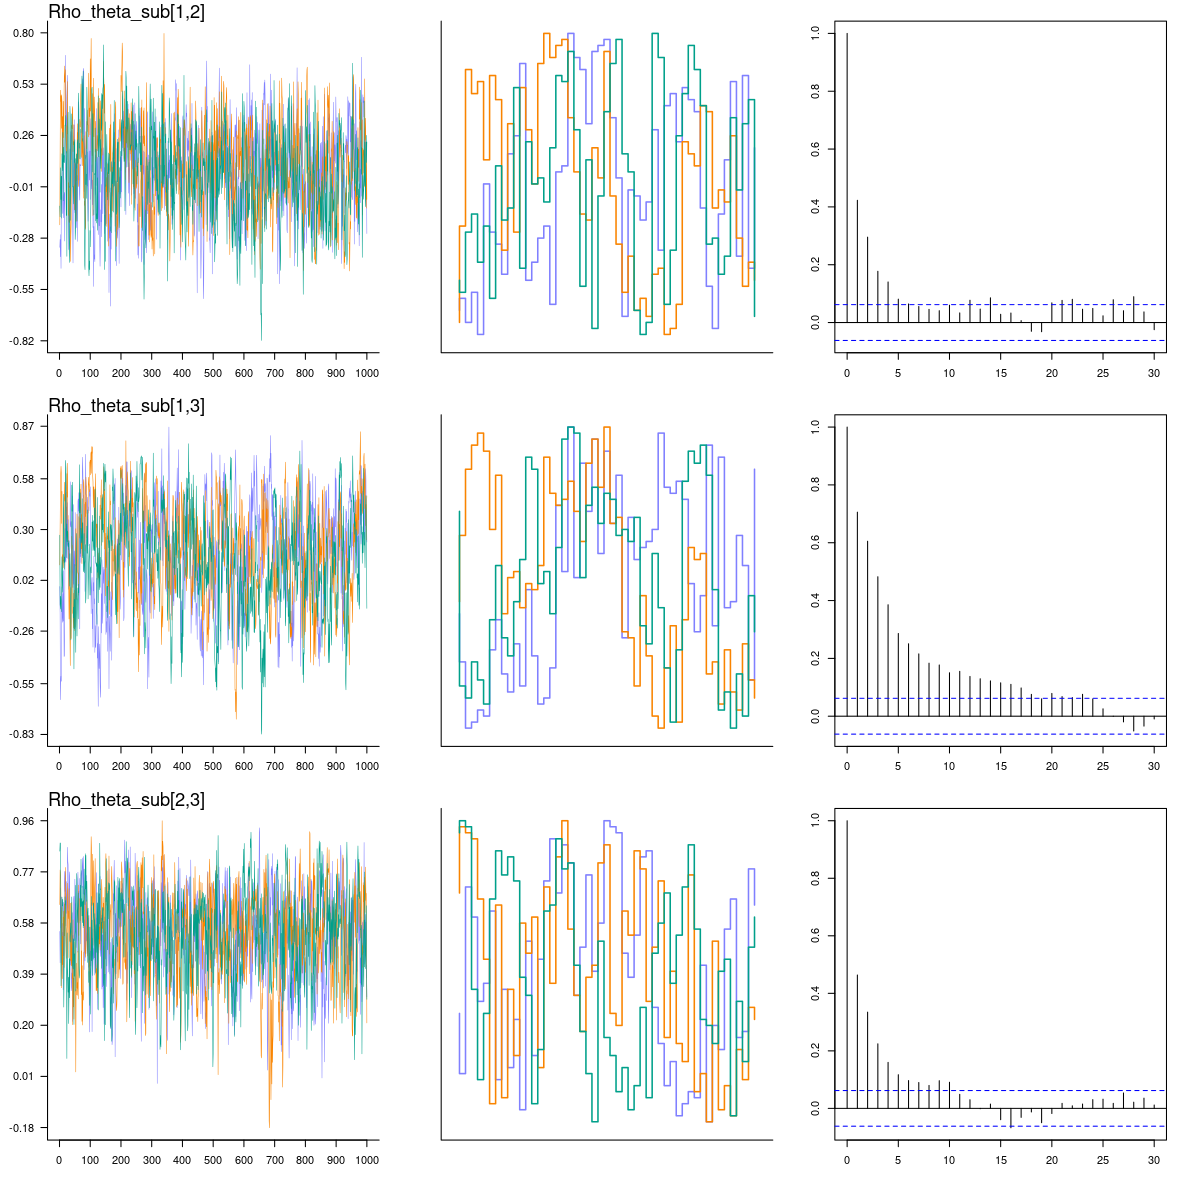
\includegraphics[width=1\linewidth]{FOLV_NC_J100_Ndata5_Rho}
	%
	\caption[First-Order latent variable model (FOLV). Non-centered parametrization. Correlation of sub-dimensions. Trace, trank and auto-correlation plots.]%
	{First-Order latent variable model (FOLV). Non-centered parametrization. Correlation of sub-dimensions: (Left) trace plot, (Middle) trank plot, (Right) auto-correlation plot.}
	\label{fig:FOLV_NC_chains8}
\end{figure}
%
\begin{figure}[H]
	\centering
	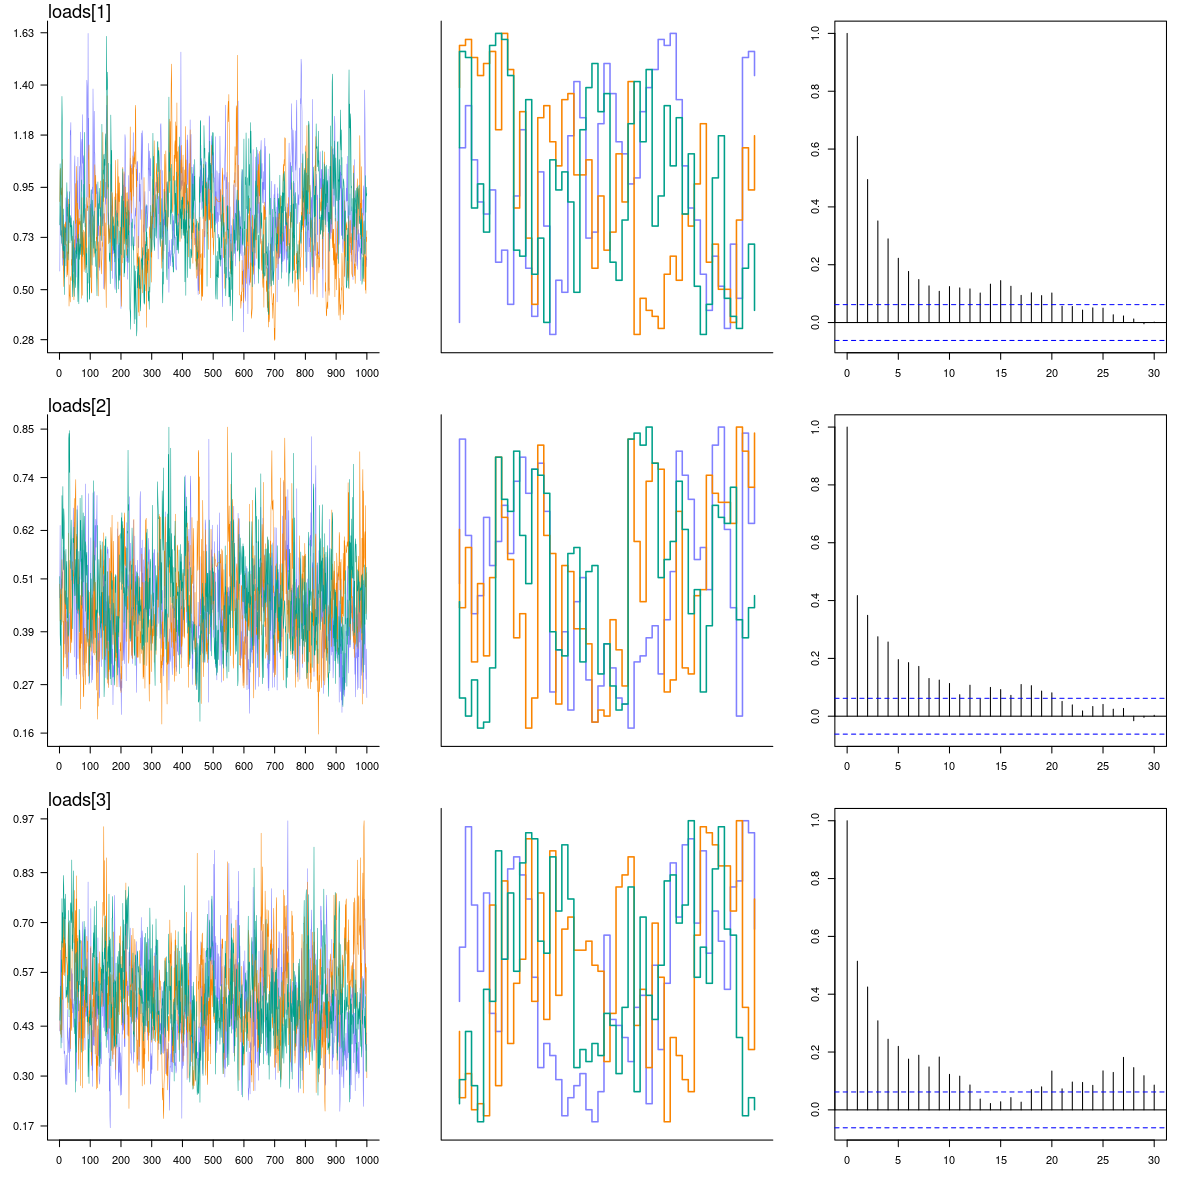
\includegraphics[width=1\linewidth]{SOLV_CE_J100_Ndata9_loads}
	%
	\caption[Second-Order latent variable model (SOLV). Centered parametrization. Loadings. Trace, trank and auto-correlation plots.]%
	{Second-Order latent variable model (SOLV). Centered parametrization. Loadings: (Left) trace plot, (Middle) trank plot, (Right) auto-correlation plot.}
	\label{fig:SOLV_CE_chains1}
\end{figure}
%
\begin{figure}[H]
	\centering
	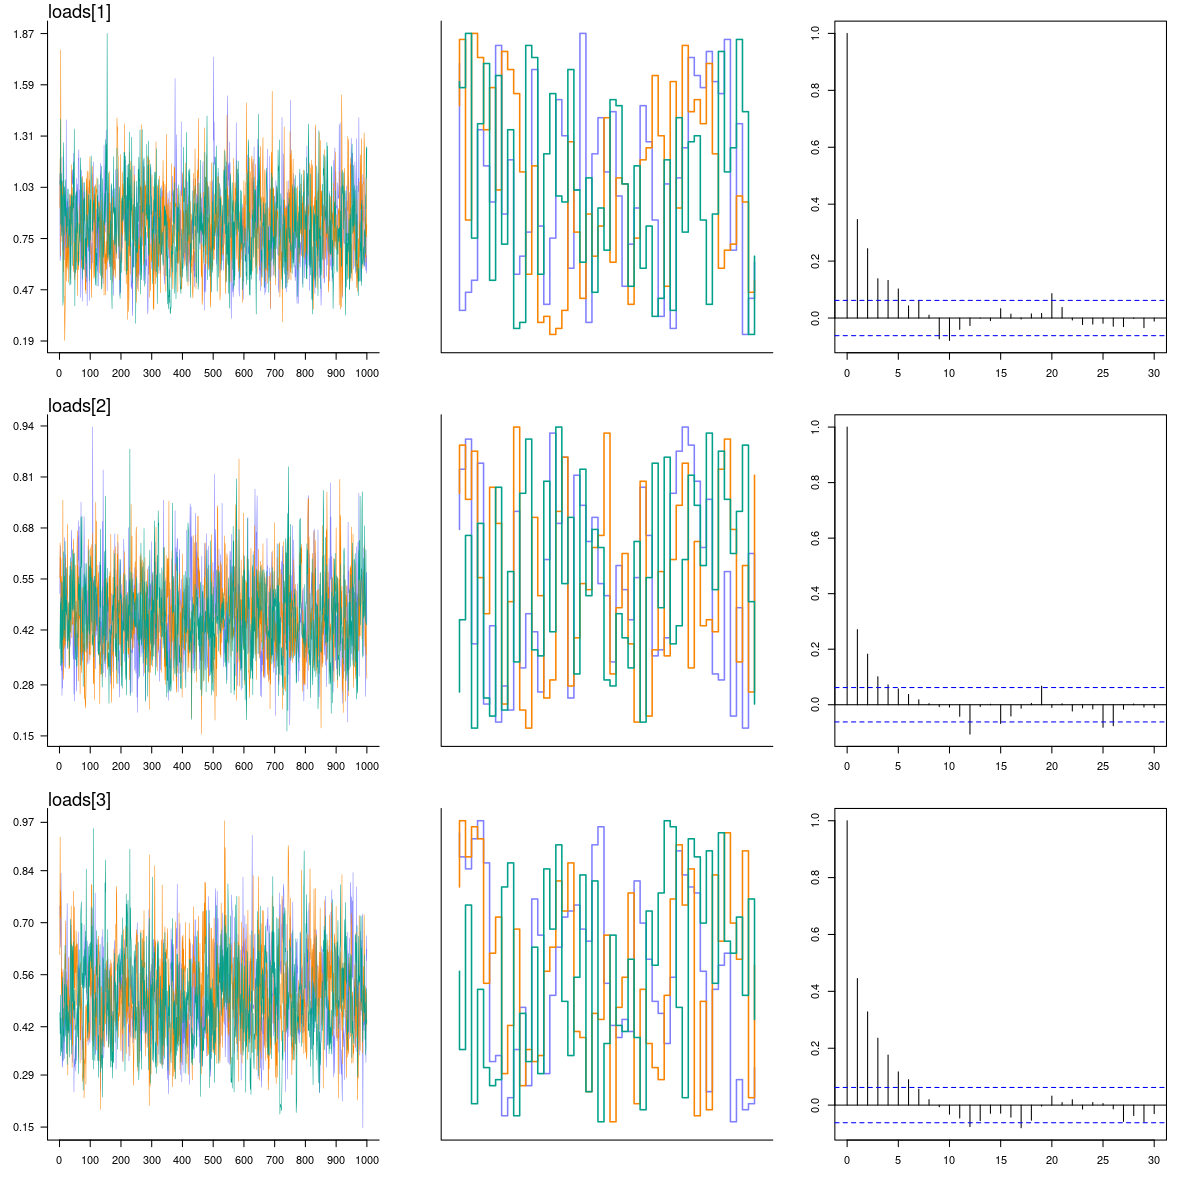
\includegraphics[width=1\linewidth]{SOLV_NC_J100_Ndata9_loads}
	%
	\caption[Second-Order latent variable model (SOLV). Non-centered parametrization. Loadings. Trace, trank and auto-correlation plots.]%
	{Second-Order latent variable model (SOLV). Non-centered parametrization. Loadings: (Left) trace plot, (Middle) trank plot, (Right) auto-correlation plot.}
	\label{fig:SOLV_NC_chains1}
\end{figure}
%
\begin{figure}[H]
	\centering
	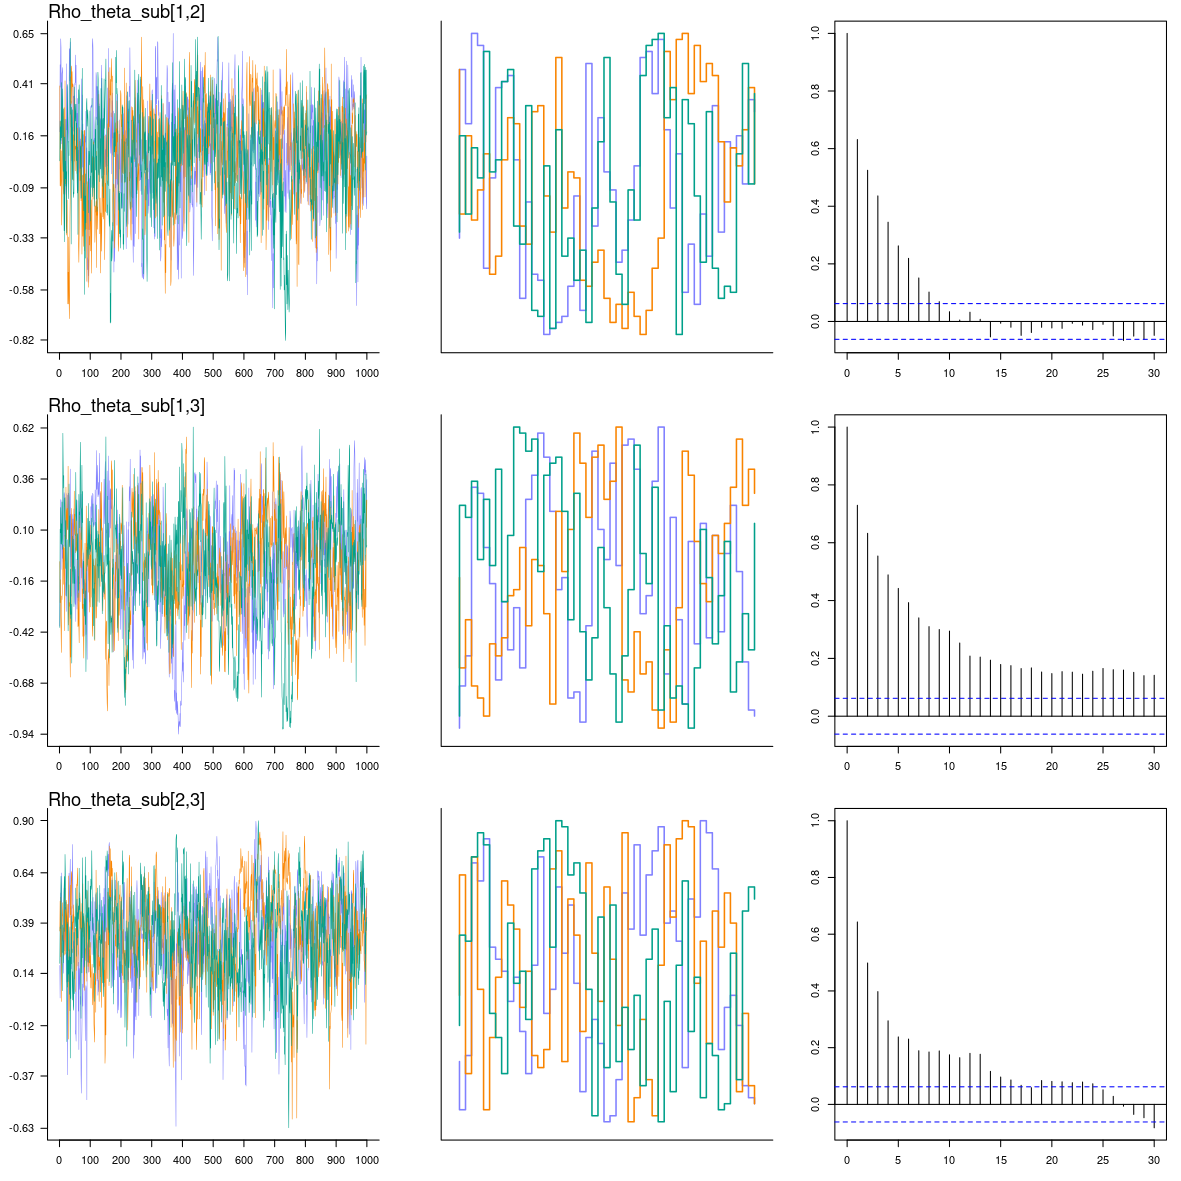
\includegraphics[width=1\linewidth]{SOLV_CE_J100_Ndata1_Rho}
	%
	\caption[Second-Order latent variable model (SOLV). Centered parametrization. Correlation of sub-dimensions. Trace, trank and auto-correlation plots.]%
	{Second-Order latent variable model (SOLV). Centered parametrization. Correlation of sub-dimensions: (Left) trace plot, (Middle) trank plot, (Right) auto-correlation plot.}
	\label{fig:SOLV_CE_chains2}
\end{figure}
%
\begin{figure}[H]
	\centering
	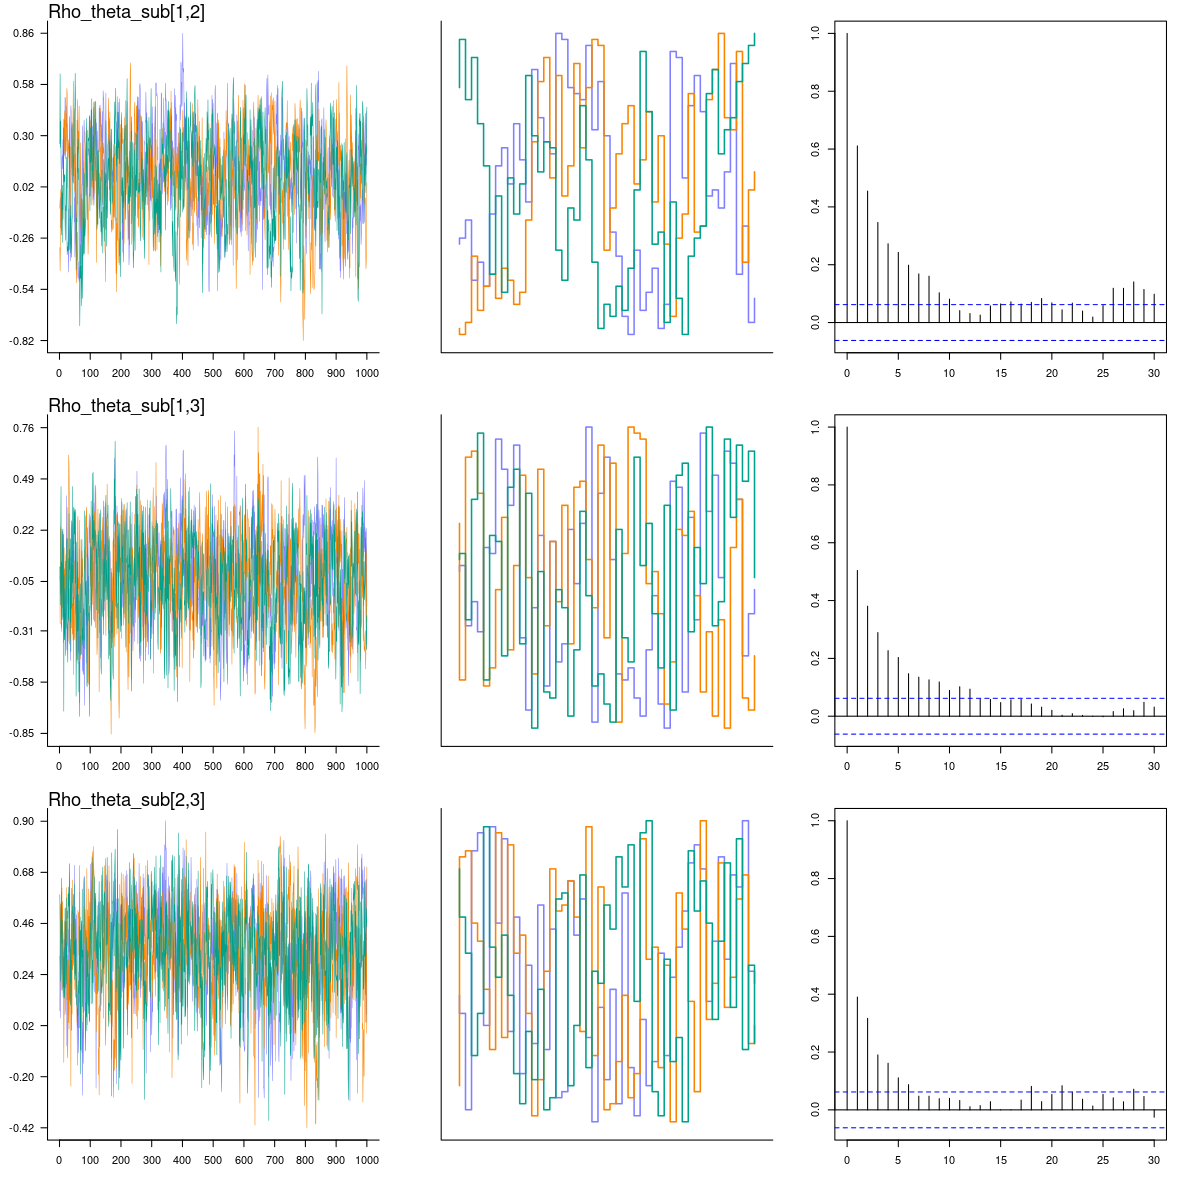
\includegraphics[width=1\linewidth]{SOLV_NC_J100_Ndata1_Rho}
	%
	\caption[Second-Order latent variable model (SOLV). Non-centered parametrization. Correlation of sub-dimensions. Trace, trank and auto-correlation plots.]%
	{Second-Order latent variable model (SOLV). Non-centered parametrization. Correlation of sub-dimensions: (Left) trace plot, (Middle) trank plot, (Right) auto-correlation plot.}
	\label{fig:SOLV_NC_chains2}
\end{figure}
%
\begin{figure}[H]
	\centering
	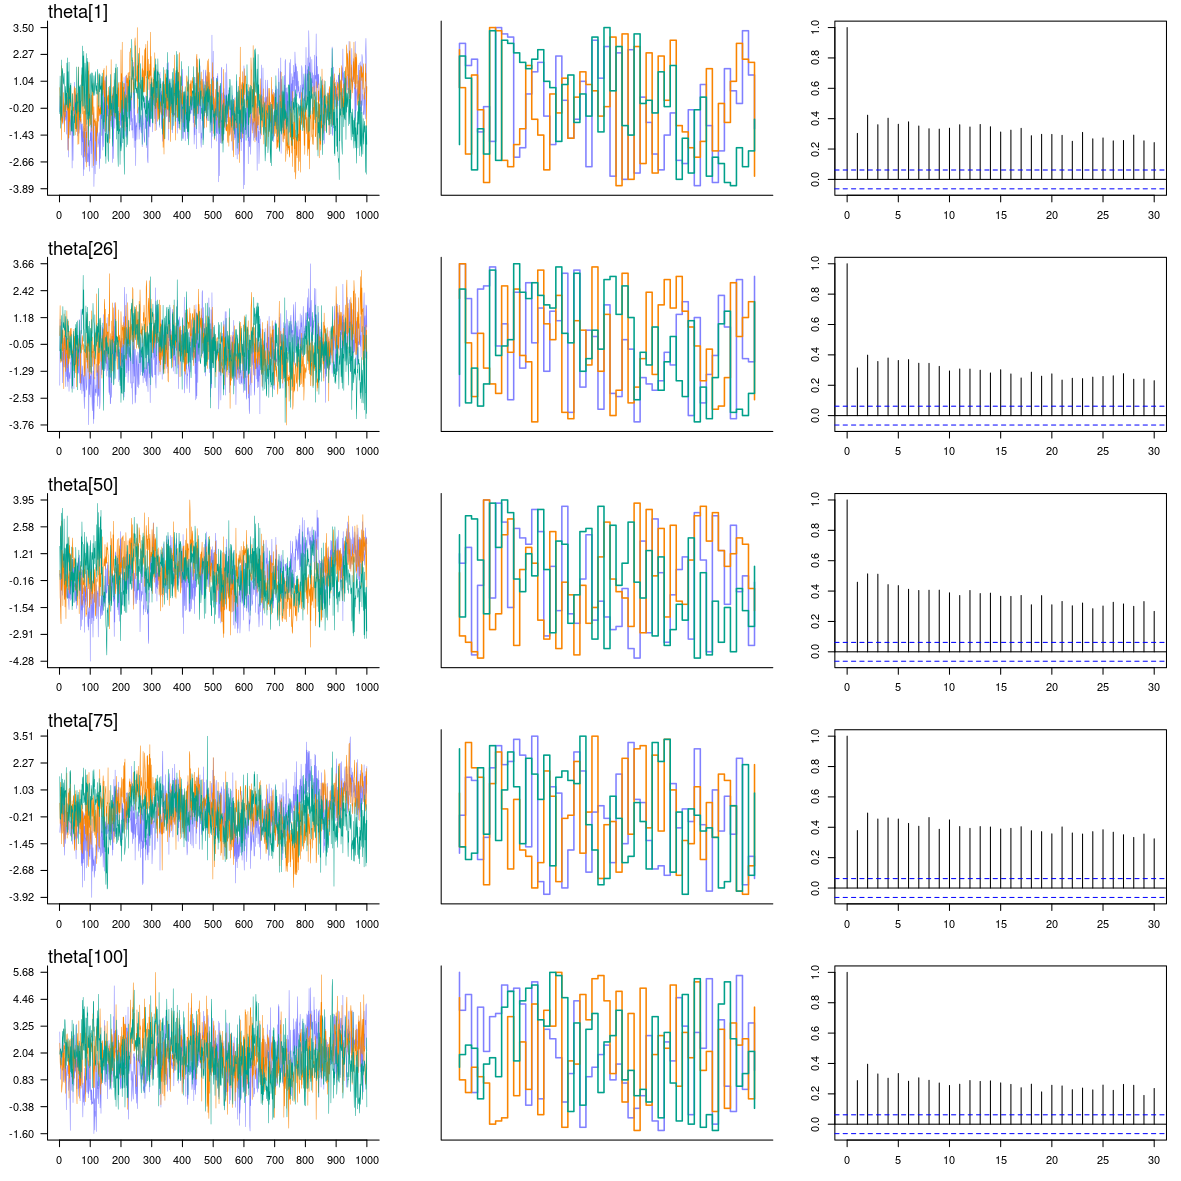
\includegraphics[width=1\linewidth]{SOLV_CE_J100_Ndata10_theta}
	%
	\caption[Second-Order latent variable model (SOLV). Centered parametrization. Highest-order dimension. Trace, trank and auto-correlation plots.]%
	{Second-Order latent variable model (SOLV). Centered parametrization. Highest-order dimension: (Left) trace plot, (Middle) trank plot, (Right) auto-correlation plot.}
	\label{fig:SOLV_CE_chains3}
\end{figure}
%
\begin{figure}[H]
	\centering
	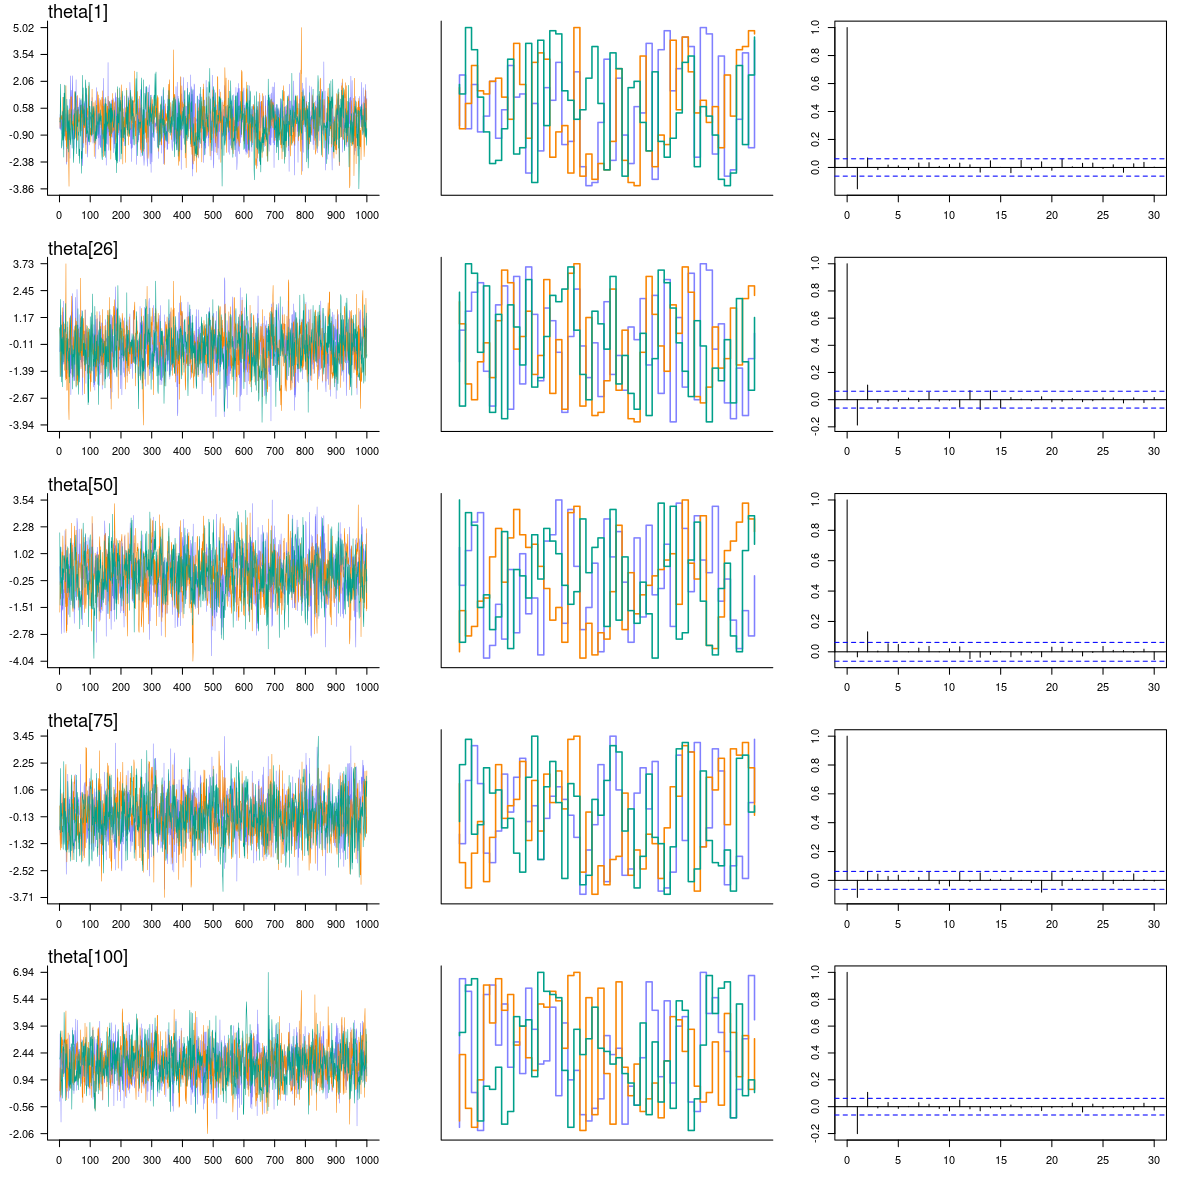
\includegraphics[width=1\linewidth]{SOLV_NC_J100_Ndata10_theta}
	%
	\caption[Second-Order latent variable model (SOLV). Non-centered parametrization. Highest-order dimension. Trace, trank and auto-correlation plots.]%
	{Second-Order latent variable model (SOLV). Non-centered parametrization. Highest-order dimension: (Left) trace plot, (Middle) trank plot, (Right) auto-correlation plot.}
	\label{fig:SOLV_NC_chains3}
\end{figure}